% import gaya yang sudah disiapkan
\documentclass{gaya}

% import berbagai variabel
%===============================================================================
% VARIABEL METADATA TUGAS AKHIR
%===============================================================================
% File ini berisi semua informasi identitas mahasiswa, pembimbing, penguji,
% dan konfigurasi dokumen. Update variabel-variabel ini sesuai data Anda.
%===============================================================================

%-------------------------------------------------------------------------------
% JUDUL TUGAS AKHIR
%-------------------------------------------------------------------------------
% Judul untuk cover (dapat multiline)
\titleind{%
  Sistem Cerdas Pelacakan Pelanggaran Helm Berbasis \textit{YOLOv8} dan \textit{ByteTrack} untuk Mendukung Analitik Data Lalu Lintas di Institut Teknologi Sumatera%
}

% Judul untuk digunakan dalam paragraf (inline)
\titleindinline{%
  Sistem Cerdas Pelacakan Pelanggaran Helm Berbasis \textit{YOLOv8} dan \textit{ByteTrack} untuk Mendukung Analitik Data Lalu Lintas di Institut Teknologi Sumatera%
}

% Judul bahasa Inggris (untuk abstrak)
\titleen{%
  Intelligent Helmet Violation Tracking System Based on \textit{YOLOv8} and \textit{ByteTrack} to Support Traffic Data Analytics at Sumatra Institute of Technology%
}

%-------------------------------------------------------------------------------
% IDENTITAS MAHASISWA
%-------------------------------------------------------------------------------
\fullname{Eggi Satria}
\newcommand{\fullnamenc}{Eggi Satria}

\idnum{122450032}
\newcommand{\idnumenc}{122450032}

%-------------------------------------------------------------------------------
% INFORMASI AKADEMIK
%-------------------------------------------------------------------------------
\degre{Sarjana Sains Data}          % Gelar yang dituju
\yearsubmit{2026}                    % Tahun pengajuan
\program{Sains Data}                 % Program studi
\dept{Sains}                         % Fakultas/Departemen

%-------------------------------------------------------------------------------
% TANGGAL PENGESAHAN
%-------------------------------------------------------------------------------
\approvaldate{25 November 2025}
\newcommand{\approvaldatenc}{25 November 2025}

%-------------------------------------------------------------------------------
% PEMBIMBING
%-------------------------------------------------------------------------------
% Pembimbing 1
\firstsupervisor{Luluk Muthoharoh, M.Si.}
\nipnrkfirst{NIP.}
\firstnip{199008172020031003}

% Pembimbing 2
\secondsupervisor{Ardika Satria, M.Si.}
\nipnrksecond{NIP.}
\secondnip{199711102024061001}

%-------------------------------------------------------------------------------
% PENGUJI
%-------------------------------------------------------------------------------
\firstexaminer{Ahmad Luky Ramdani, S.Kom., M.Kom}   % Penguji 1
\secondexaminer{}     % Penguji 2

%-------------------------------------------------------------------------------
% KOORDINATOR PROGRAM STUDI
%-------------------------------------------------------------------------------
\headofdepartment{Tirta Setiawan, S.Pd., M.Si.}
\nipnrkhead{NIP.}
\headnip{199008222022031003}


%-------------------------------------------------------------------------------
% KONFIGURASI TAHAPAN TUGAS AKHIR
%-------------------------------------------------------------------------------
% Pilihan: sempro | semhas | sidang | final
% - sempro: Seminar Proposal
% - semhas: Seminar Hasil
% - sidang: Sidang Tugas Akhir
% - final:  Dokumen Final (untuk pengumpulan)
\def\tahapan{semhas}

%===============================================================================
% CATATAN PENGGUNAAN:
%===============================================================================
% 1. Pastikan semua nama ditulis lengkap dengan gelar
% 2. Format NIP tanpa spasi atau tanda hubung
% 3. Keywords pisahkan dengan koma, maksimal 5-7 kata kunci
% 4. Ubah \tahapan sesuai progres TA Anda
% 5. Untuk judul panjang, gunakan % di akhir baris untuk menghindari spasi
%===============================================================================

\input{pustaka/jenis-dokumen.tex}

% pemenggalan kata
\input{pustaka/tanda-hubung.tex}

% Isi keseluruhan dokumen
\begin{document}

% Sampul luar bahasa indonesia
\cover
\newpage

% Nomor halaman pembuka dimulai dari sini
\pagenumbering{roman}

% % Sampul dalam bahasa indonesia
% \coverdalam
% \newpage

% % Halaman pengesahan
% \approvalpage
% \cleardoublepage

% % Halaman orisinalitas
% \originalitypage
% \cleardoublepage

% % Halaman publikasi
% \publicationpage
% \cleardoublepage

% !TEX root = ../main.tex
\begin{abstractind}
  \justifying
  Peningkatan mobilitas kendaraan roda dua di lingkungan perguruan tinggi meningkatkan risiko keselamatan, khususnya terkait ketidakpatuhan penggunaan helm. Pengawasan manual konvensional dinilai kurang terukur dan belum mampu menyediakan wawasan spasiotemporal yang presisi untuk evaluasi kebijakan. Penelitian ini bertujuan merancang dan mengevaluasi arsitektur sistem pengawasan cerdas berbasis aliran video waktu nyata (\textit{real-time video streaming}) secara ujung ke ujung (\textit{end-to-end}). Arsitektur yang diusulkan mengintegrasikan model YOLOv8 untuk ekstraksi fitur spasial, ByteTrack untuk pelacakan multiobjek, serta filter \textit{Intersection over Area} (IoA) dan konfirmasi temporal berbasis \textit{N-Frame} untuk mereduksi deteksi palsu. Aliran peristiwa kemudian didistribusikan melalui Apache Kafka dan Apache Spark Structured Streaming ke \textit{data mart} PostgreSQL sebelum divisualisasikan pada dasbor interaktif Grafana. Hasil evaluasi eksperimental menunjukkan bahwa model deteksi mencapai \textit{Mean Average Precision} (mAP@50) sebesar 91,4\%. Sistem pemrosesan tepi beroperasi stabil dengan \textit{throughput} 18,9 FPS dan latensi inferensi 53 milidetik, sementara pialang pesan mencatat tingkat keberhasilan pengiriman 100\% dengan median latensi 2,65 milidetik. Pengujian operasional menggunakan data lapangan selama 10 jam (07.00--17.00 WIB) memvalidasi keandalan \textit{pipeline} dalam menyaring 11.172 deteksi mentah menjadi 113 kejadian pelanggaran aktual. Analisis visual pada dasbor berhasil memetakan distribusi kepadatan bimodal secara empiris, dengan puncak anomali ekstrem terekam pada pukul 14.45--15.15 WIB yang berkorelasi dengan faktor cuaca dan dinamika pergantian kelas. Secara keseluruhan, infrastruktur terintegrasi ini mentransformasi metode pengawasan reaktif menjadi instrumen Sistem Pendukung Keputusan (\textit{Decision Support System}) yang proaktif untuk mengoptimalkan efisiensi perencanaan patroli keselamatan di lingkungan kampus.

\noindent
\textbf{Kata kunci:} ByteTrack, \textit{Data Mart}, Pelanggaran Helm, YOLOv8 % masukkan keyword
\end{abstractind}

\cleardoublepage

% % Abstrak Bahasa Inggris
% % !TEX root = ../main.tex
\begin{abstracteng}
  \justifying
  The increasing mobility of two-wheeled vehicles in university environments triggers an escalation of safety risks, particularly non-compliance with helmet usage. Conventional manual surveillance is considered unscalable and fails to provide precise spatio-temporal insights for policy evaluation. This study aims to design and evaluate an end-to-end smart surveillance system architecture based on real-time video streaming. The proposed architecture integrates the YOLOv8 model for spatial feature extraction, ByteTrack for multi-object tracking, as well as \textit{Intersection over Area} (IoA) filters and \textit{N-Frame} temporal confirmation to reduce false detections. The event stream is then distributed through Apache Kafka and Apache Spark Structured Streaming into a PostgreSQL \textit{data mart}, before being visualized on an interactive Grafana dashboard. Experimental evaluation results demonstrate that the inference model achieves a \textit{Mean Average Precision} (mAP@50) of 91.4\%. The edge processing system operates stably with a \textit{throughput} of 18.9 FPS and an inference latency of 53 milliseconds, while the message broker records a 100\% delivery success rate with a median latency of 2.65 milliseconds. Operational testing using 10 hours of field data (07.00--17.00 local time) validates the \textit{pipeline}'s reliability in filtering 11,172 raw detections into 113 actual violation events. Visual analysis on the dashboard empirically maps a bimodal density distribution, with an extreme anomaly peak recorded at 14:45--15:15 WIB, which is correlated with weather factors and class transition dynamics. Overall, this integrated infrastructure transforms reactive surveillance methods into a proactive \textit{Decision Support System} instrument that optimizes the efficiency of safety patrol planning in the campus environment.

  \bigskip
  \noindent
  \textbf{Keywords:} YOLOv8, ByteTrack, Stream Processing, Data Mart, Traffic Safety.
\end{abstracteng}

% \cleardoublepage

% % Motto
% \motto
\begin{centering}
\vfill
\emph{“Be kind, Be forgiving, but never be a pushover.”\\[.6cm]}
\vfill
\end{centering}

% \cleardoublepage

% % Persembahan
% \acknowledgment
\begin{centering}
\vfill
\emph{Untuk Mama tercinta di kampung halaman,\\yang telah berjuang keras menyekolahkan Eggi,\\dan keluarga tercinta yang selalu mendukung,\\dengan cinta abadi dan doa yang tak pernah padam.\\[.5cm]}
\vfill
\end{centering}

% \cleardoublepage

% % Kata pengantar
% %-----------------------------------------------------------------
%Di sini awal masukan untuk Prakata
%------------------------------------------------------------
\preface
\justifying
\noindent Puji syukur penulis panjatkan ke hadirat Allah SWT atas berkah dan rahmat-Nya sehingga skripsi ini dapat terselesaikan dengan baik. Skripsi ini dibuat untuk menyelesaikan pendidikan jenjang sarjana pada Institut Teknologi Sumatera. Penyusunan skripsi ini banyak mendapat bantuan dan dukungan dari berbagai pihak sehingga dalam kesempatan ini, dengan penuh kerendahan hati, penulis mengucapkan terima kasih kepada:
\begin{enumerate}
\item{Prof. Dr. I Nyoman Pugeg Aryantha selaku Rektor Institut Teknologi Sumatera,}
\item{Dr. Ikah Ning Prasetiowati Permanasari, S.Si., M.Si. selaku Dekan Fakultas Sains Institut Teknologi Sumatera,}
\item{Tirta Setiawan, S.Pd., M.Si. selaku Koordinator Program Studi,}
\item{Luluk Muthoharoh, M.Si. selaku dosen wali akademik dan juga pembimbing penelitian yang telah memberikan arahan dan bimbingan selama perkuliahan,}
\item{Ardika Satria, M.Si. selaku dosen pembimbing skripsi yang telah banyak memberikan bimbingan, saran, serta motivasi kepada penulis dalam penyusunan skripsi ini,} 
\item{Teman-teman seperjuangan selama perkuliahan di Institut Teknologi Sumatera, khususnya teman-teman angkatan 2022 Program Studi Sains Data,}
\end{enumerate}

Penulis menyadari bahwa penyusunan skripsi ini jauh dari sempurna.
Akhir kata penulis mohon maaf yang sebesar-besarnya apabila ada kekeliruan di dalam penulisan skripsi ini.



\vspace{0.5cm}

\begin{flushright}
\begin{tabular}{p{3.5cm}l}
&Lampung Selatan, \approvaldatenc \\[1.5cm]
&\textbf{\fullnamenc}
\end{tabular}
\end{flushright}
% \cleardoublepage

% Daftar Isi
\addcontentsline{toc}{chapter}{DAFTAR ISI}
\tableofcontents

% Daftar Gambar
\phantomsection%<---
\addcontentsline{toc}{chapter}{DAFTAR GAMBAR}
\listoffigures

% Daftar Tabel
\phantomsection%<---
\addcontentsline{toc}{chapter}{DAFTAR TABEL}
\listoftables

% % Daftar Singkatan
% \include{lainnya/daftar-singkatan.tex}

% % Daftar Simbol
% \include{lainnya/daftar-simbol.tex}

\newpage

% Nomor halaman isi dimulai dari sini
\pagenumbering{arabic}

% Bab 1 pendahuluan
% !TEX root = ../main.tex
\chapter{PENDAHULUAN}

\section{Latar Belakang}
\label{section:latarbelakang}

% === Paragraf 1: Visi Itera dan Daya Tarik Forest Campus ===
Institut Teknologi Sumatera (Itera) memiliki visi untuk menjadi perguruan
tinggi teknologi yang unggul dengan lingkungan kampus yang nyaman, aman, dan
berwawasan lingkungan \cite{itera2019renstra}. Salah satu implementasinya
adalah konsep \textit{forest campus}. Konsep ini tidak hanya menata ruang
hijau, tetapi juga menekankan keberlanjutan, ketertiban, dan kualitas hidup
sivitas akademika. Dalam praktiknya, pengembangan \textit{forest campus}
terhubung dengan konsep \textit{smart campus}. Konsep ini memanfaatkan sistem
digital, Internet of Things (IoT), dan kecerdasan buatan untuk meningkatkan
efisiensi operasional, pengalaman pengguna, dan keselamatan
\cite{Polin2023SmartCampus}. Kombinasi nilai ekologis dan teknologi tersebut
memperkuat citra Itera dan meningkatkan daya tariknya bagi calon mahasiswa.

% === Paragraf 2: Masalah Pertumbuhan dan Tantangan Mobilitas ===
Daya tarik tersebut berdampak pada peningkatan jumlah mahasiswa baru setiap
tahun. Data akademik dan statistik mahasiswa menunjukkan tren kenaikan
penerimaan mahasiswa dari tahun ke tahun \cite{itera2025dashboard}.
Pertumbuhan ini berkorelasi dengan meningkatnya
penggunaan kendaraan pribadi, terutama sepeda motor
\cite{purwanti2018analisisitenas}. Berbagai studi menunjukkan bahwa kenaikan
populasi kampus meningkatkan volume transportasi dan konsumsi energi
\cite{rachmadian2024kesadaran}. Studi tersebut juga menekankan keterlibatan
mahasiswa dalam inisiatif transportasi dan energi berkelanjutan di lingkungan
perguruan tinggi \cite{rachmadian2024kesadaran}. Itera telah memulai
pengembangan transportasi umum melalui Smart BRT \cite{antaranews2025brt}.
Kapasitas dan jangkauannya masih terbatas \cite{antaranews2025brt}. Kondisi tersebut meningkatkan potensi pelanggaran lalu lintas, salah satunya
ketidakpatuhan penggunaan helm. Isu ini juga menjadi perhatian nasional.
Penelitian lintas-seksional di lingkungan universitas menunjukkan bahwa 40,8\%
mahasiswa pengendara sepeda motor tidak menggunakan helm secara konsisten
\cite{safitri2020gambaran}. Penelitian lain mengidentifikasi beberapa penyebab
utama kepatuhan helm pada remaja, meliputi faktor keluarga, ekonomi,
individu, dan sosial-budaya \cite{nobrihas2023kepatuhan}. Untuk menekan risiko kecelakaan, Itera telah
menjalankan program kolaborasi keselamatan berkendara bersama mitra
eksternal. Di perguruan tinggi lain, pedoman berlalu lintas juga ditetapkan
secara formal melalui peraturan rektor
\cite{iteranews2024kolaborasi,its2025pedoman}. Namun, tantangan utama masih berada pada
sistem penegakan aturan. Pengawasan saat ini masih mengandalkan satuan
pengamanan (Satpam) secara manual, sehingga belum dapat mencakup seluruh area
kampus secara berkelanjutan dan tetap rentan terhadap kesalahan manusia.
Pendekatan ini juga belum menghasilkan data kuantitatif yang konsisten.
Akibatnya, informasi penting seperti lokasi \textit{hotspot}, waktu puncak,
dan frekuensi pelanggaran belum terdokumentasi dengan baik. Kondisi ini
menyulitkan Unit Pelaksana Teknis Keselamatan, Kesehatan Kerja, dan
Lingkungan (UPT K3L) Itera dalam merumuskan intervensi yang tepat sasaran dan
berbasis bukti.

% === Paragraf 4: Solusi yang Diusulkan - Sistem Cerdas YOLOv8 + ByteTrack ===
Penelitian ini mengusulkan sistem visi komputer untuk mendeteksi dan
menganalisis pelanggaran penggunaan helm di lingkungan kampus Itera. Rancangan
sistem mengintegrasikan YOLOv8 sebagai model deteksi objek. ByteTrack digunakan
sebagai algoritma pelacakan multiobjek untuk menjaga konsistensi identitas
pengendara antar-\textit{frame}. Kombinasi ini efektif untuk analisis lalu lintas berbasis
video pada skenario dinamis dengan banyak objek bergerak \cite{liu2025vehicle}.
Berbeda dengan pendekatan yang berhenti pada identifikasi visual, penelitian
ini mentransformasikan keluaran inferensi menjadi aliran peristiwa
(\textit{event stream}). Aliran ini memuat konteks spasial dan temporal, seperti
waktu kejadian, titik kamera, identitas objek, dan status pelanggaran. Setiap
peristiwa dicatat sebagai metadata terstruktur dan disimpan dalam \textit{data mart}.
Penyimpanan ini mendukung analisis historis, nonvolatil, dan berorientasi
analitik. Dengan pendekatan ini, sistem berfungsi sebagai alat deteksi otomatis.
Sistem juga menjadi fondasi analitik jangka panjang untuk mengidentifikasi
\textit{hotspot} pelanggaran dan menentukan waktu rawan. Hasilnya mendukung
pengambilan keputusan keselamatan berbasis data dalam kerangka
\textit{smart campus}.

\section{Rumusan Masalah}
\label{section:rumusanmasalah}

Berdasarkan latar belakang yang telah diuraikan, rumusan masalah penelitian
ini adalah sebagai berikut:

\begin{enumerate}
  \item Bagaimana merancang dan melatih YOLOv8 untuk mendeteksi pengendara sepeda motor berhelm dan tanpa helm pada video CCTV kampus secara andal?

  \item Bagaimana mengintegrasikan YOLOv8 dan ByteTrack pada pemrosesan video \textit{real-time} agar inferensi menjadi \textit{event stream} dengan konteks spasial dan temporal?

  \item Bagaimana merancang skema \textit{data mart} untuk menyimpan peristiwa pelanggaran helm secara sistematis agar mendukung analisis pola lalu lintas dan tren keselamatan di Itera?
\end{enumerate}

\section{Tujuan Penelitian}
\label{section:tujuanpenelitian}

Tujuan penelitian ini adalah sebagai berikut:

\begin{enumerate}
  \item Mengembangkan dan melatih YOLOv8 untuk mendeteksi pengendara sepeda motor berhelm dan tanpa helm pada lingkungan kampus.

  \item Mengimplementasikan integrasi YOLOv8 dan ByteTrack pada pemrosesan video \textit{real-time} untuk menghasilkan \textit{event stream} pelanggaran helm dengan konteks spasial dan temporal.

  \item Merancang dan mengimplementasikan \textit{data mart} analitik sebagai bagian dari arsitektur \textit{data warehouse} untuk menyimpan hasil deteksi pelanggaran helm secara historis. Hasilnya mendukung analisis pola lalu lintas dan keputusan keselamatan berbasis data di Itera.

\end{enumerate}

\section{Batasan Penelitian}
\label{section:batasanpenelitian}

Untuk memastikan penelitian tetap fokus dan dapat diselesaikan dalam kurun
waktu yang ditetapkan, ruang lingkup penelitian dibatasi sebagai berikut:

\begin{enumerate}
  \item Penelitian difokuskan pada deteksi dan analisis pelanggaran penggunaan helm oleh pengendara sepeda motor. Pelanggaran lain, seperti kecepatan, parkir liar, atau rambu, tidak termasuk dalam cakupan penelitian.

  \item Penelitian berfokus pada analisis historis dan agregatif dari aliran peristiwa pelanggaran helm. Sistem tidak dirancang untuk memprediksi kejadian atau memberikan rekomendasi kebijakan secara otomatis.

  \item YOLOv8 digunakan sebagai komponen untuk mengekstraksi informasi visual dari data video. Penelitian tidak membahas modifikasi arsitektur internal YOLOv8, perbandingan dengan detektor lain, maupun optimasi pada tingkat algoritmik.

  \item Pengumpulan dan pengujian data dilakukan dalam rentang waktu tertentu, yaitu pada 5 Februari 2026 dengan jendela observasi pukul 07.00--17.00 WIB.

  \item Penelitian tidak melakukan perbandingan eksperimental antara arsitektur streaming dan non-streaming. Fokus berada pada perancangan dan evaluasi sistem analitik end-to-end berbasis peristiwa.

  \item Evaluasi operasional menggunakan sumber komputasi perangkat keras yang tersedia pada satu mesin pengujian. Keterbatasan kapasitas CPU, memori, dan GPU pada lingkungan eksperimen menyebabkan pengujian multi-kamera skala besar belum dapat dijalankan sebagai operasi produksi penuh.
\end{enumerate}

% Sub bab lain dapat ditambahkan, misalnya:
%\section{Manfaat Penelitian}
%\section{Hipotesis}


% % Bab 2 tinjauan pustaka
\include{bab/2-tinjauan-pustaka.tex}

% % Bab 3 metodologi penelitian
% !TEX root = ../main.tex
\chapter{METODOLOGI PENELITIAN}
\label{chap:metodologi}

\section{Lingkungan Pengembangan}
Pengembangan dan pengujian sistem dilakukan pada satu unit laptop dengan spesifikasi perangkat keras yang ditunjukkan pada Tabel~\ref{tab:spek-hardware}.

\begin{table}[h]
  \centering
  \caption{Spesifikasi Perangkat Keras}
  \label{tab:spek-hardware}
  \footnotesize
  \setlength{\tabcolsep}{4pt}
  \begin{tabular}{p{0.34\textwidth} p{0.5\textwidth}}
    \toprule
    \textbf{Komponen} & \textbf{Spesifikasi} \\
    \midrule
    Prosesor            & AMD Ryzen 5 7535HS (6 Core / 12 Thread, 3{,}3 GHz) \\
    Memori (RAM)        & 16 GB DDR5 \\
    Penyimpanan         & 512 GB NVMe SSD \\
    GPU                 & AMD Radeon Graphics (Integrated) \\
    \bottomrule
  \end{tabular}
\end{table}

\section{Deskripsi Data}
Subbab ini menjelaskan deskripsi data yang digunakan dalam penelitian, meliputi jenis dan sumber data, proses anotasi, serta strategi augmentasi. Uraian rinci setiap aspek disajikan pada subsubbab berikutnya sebagai dasar pembentukan dataset dan evaluasi model.
\subsection{Jenis dan Sumber Data}
Data yang digunakan dalam penelitian ini dikategorikan menjadi dua jenis utama berdasarkan asal dan perannya dalam sistem, yaitu data primer dan data sekunder.

\begin{enumerate}[a.]
  \item Data Primer:
    Data primer berupa rekaman video CCTV yang diperoleh dari Unit K3L Institut Teknologi Sumatera (Itera) berdasarkan izin resmi tertulis. Data yang digunakan merupakan rekaman luring (\textit{non-real-time}) dari satu kamera CCTV yang terpasang di gerbang utama kampus. Rekaman mencakup periode pengamatan satu hari, yaitu 5 Februari 2026, dengan rentang waktu perekaman pukul 07.00 hingga 17.00 WIB.

    Rekaman ini merepresentasikan arus lalu lintas utama kendaraan bermotor yang masuk dan keluar area kampus, sehingga relevan untuk analisis pelanggaran penggunaan helm di lingkungan kampus.

  \item Data Sekunder:
    Untuk mendukung pelatihan dan evaluasi model deteksi objek berbasis YOLOv8, penelitian ini menggunakan data sekunder berupa \textit{ITERA Helmet Dataset}. Dataset ini dibangun dari data primer melalui ekstraksi \textit{frame} secara selektif. Pengambilan \textit{frame} dilakukan berdasarkan kondisi visual yang memadai untuk deteksi objek, sehingga diperoleh 390 \textit{frame} yang representatif. Dataset kemudian dianotasi secara manual dengan tiga kelas target: \texttt{DRIVER\_HELMET}, \texttt{DRIVER\_NO\_HELMET}, dan \texttt{MOTORCYCLE}.
\end{enumerate}

\subsection{Anotasi Data}
Anotasi dilakukan secara manual untuk membentuk data \textit{ground truth} pada setiap \textit{frame} hasil ekstraksi. Objek pengendara dan sepeda motor diberikan \textit{bounding box}. Pengendara dilabeli \texttt{DRIVER\_HELMET} atau \texttt{DRIVER\_NO\_HELMET}, sedangkan sepeda motor dilabeli \texttt{MOTORCYCLE} sebagai konteks pelacakan. Skema anotasi diterapkan secara konsisten pada seluruh data (Gambar~\ref{fig:contoh_anotasi}), kemudian diverifikasi dan diekspor ke format YOLO.

\begin{figure}[htpb]
  \centering
  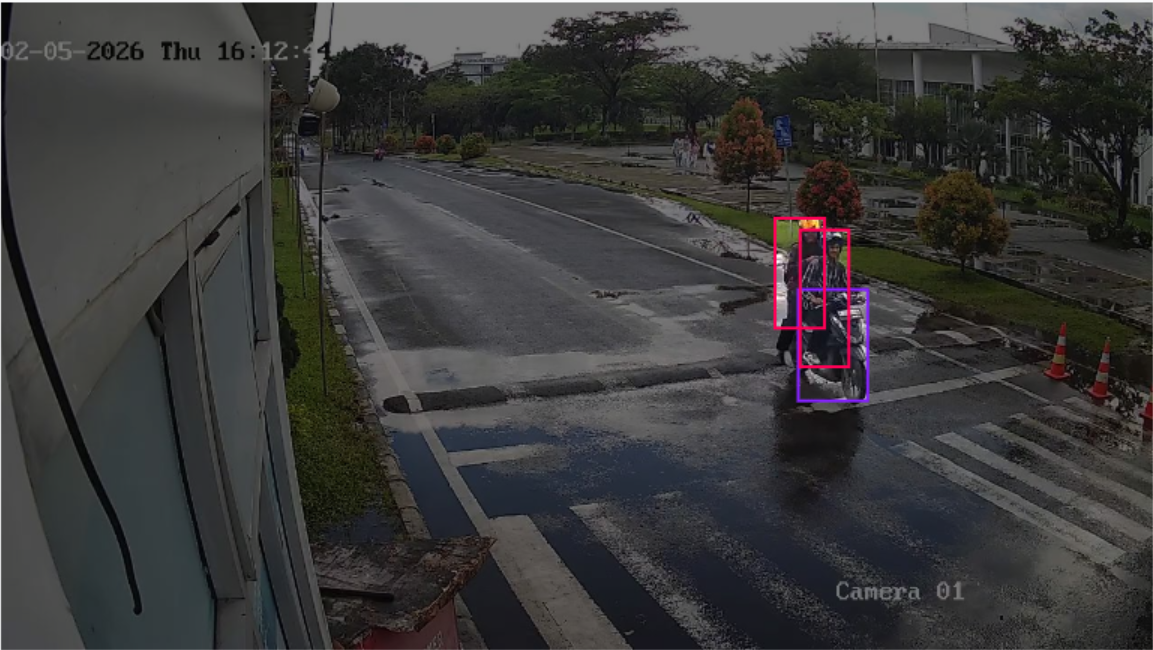
\includegraphics[width=0.8\textwidth]{gambar/data_anotation.png}
  \caption{Contoh anotasi \textit{bounding box} pada pengendara dan sepeda motor dari tangkapan layar CCTV.}
  \label{fig:contoh_anotasi}
\end{figure}

\subsection{Augmentasi Data}
Augmentasi diterapkan hanya pada data latih untuk mengurangi \textit{overfitting} dan meningkatkan generalisasi model. Transformasi meliputi rotasi, \textit{shear}, perubahan eksposur, \textit{blur}, \textit{noise}, dan \textit{motion blur}. Rentang parameter dipilih secara moderat agar variasi visual meningkat tanpa mengubah makna objek. Data validasi dan data uji tidak diaugmentasi untuk menjaga objektivitas evaluasi. Rincian parameter disajikan pada Tabel~\ref{tab:augmentasi}.

\begin{table}[htpb]
  \centering
  \caption{Parameter Augmentasi Data}
  \label{tab:augmentasi}
  \begin{tabular}{ll}
    \toprule
    \textbf{Teknik Augmentasi} & \textbf{Parameter} \\
    \midrule
    Rotation & Antara $-8^\circ$ dan $+8^\circ$ \\
    Shear & $\pm 10^\circ$ horizontal, $\pm 10^\circ$ vertikal \\
    Exposure & Antara $-10\%$ dan $+10\%$ \\
    Blur & Hingga 1,4 piksel \\
    Noise & Hingga 1,09\% dari total piksel \\
    Motion Blur & \textit{Length} 10 px, \textit{Angle} $0^\circ$, \textit{Frames} 1 \\
  \bottomrule
  \end{tabular}
\end{table}

\section{Arsitektur Sistem}
Sistem dibangun dengan \textit{Kappa Architecture} \cite{kreps2014questioning}, yang menempatkan pemrosesan aliran data sebagai jalur utama. Arsitektur ini terdiri atas enam lapisan utama dan ditunjukkan pada Gambar~\ref{fig:architecture}. Secara ringkas, aliran data dimulai dari lapisan \textit{Data Source} sebagai sumber video CCTV yang telah disertai identitas kamera, resolusi, dan posisi geospasial, lalu diteruskan ke lapisan \textit{Ingestion \& Edge Intelligence} untuk akuisisi, pra-pemrosesan \textit{frame}, serta penambahan stempel waktu dan metadata teknis. Data berikutnya dikirim ke lapisan \textit{Buffering} menggunakan Apache Kafka sebagai \textit{message broker} agar aliran data tetap andal, skalabel, dan berurutan per kamera. Setelah itu, lapisan \textit{Stream Processing} memproses \textit{event} secara \textit{real-time} dengan Apache Spark Structured Streaming melalui validasi skema, deduplikasi, dan agregasi singkat sebelum hasilnya disimpan pada lapisan \textit{Persistence} ke dalam \textit{data mart} berdesain skema bintang dengan mekanisme \textit{upsert}. Pada tahap akhir, lapisan \textit{Presentation} memanfaatkan Grafana Dashboard untuk menyajikan hasil analitik secara \textit{real-time} melalui visualisasi yang mendukung pemantauan dan pengambilan keputusan operasional secara cepat dan terarah.

\begin{figure}[H]
  \centering
  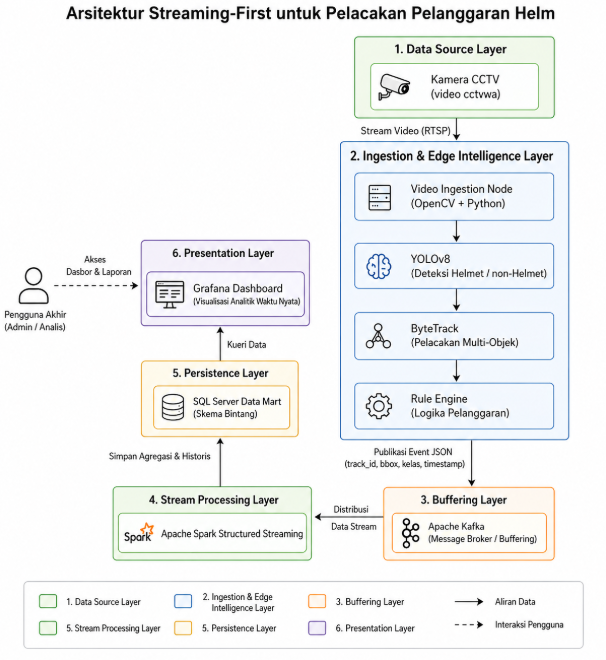
\includegraphics[width=1\textwidth]{gambar/kappa_arsitektur_helm.png}
  \caption{Arsitektur Sistem Streaming-First Pelacakan Pelanggaran Helm}
  \label{fig:architecture}
\end{figure}
\section{Perancangan Model YOLOv8 dan ByteTrack}
Bagian ini menjelaskan perancangan model deteksi dan pelacakan, mulai dari proses pelatihan YOLOv8 hingga integrasi ByteTrack pada tahap inferensi.

\subsection{Pelatihan Model YOLOv8}
Model YOLOv8s yang telah dilatih pada dataset COCO disesuaikan ulang melalui proses \textit{fine-tuning} menggunakan dataset kustom Itera pada \textit{framework} Ultralytics. Proses ini menghasilkan berkas model \textit{best.pt} dengan bobot optimal untuk inferensi pada lapisan \textit{Ingestion \& Edge Intelligence}.

\section{Logika Deteksi Pelanggaran Helm}

Sistem mengintegrasikan model deteksi objek YOLOv8 dan algoritma pelacakan multiobjek ByteTrack untuk mengidentifikasi pengendara yang menggunakan dan tidak menggunakan helm.

Rangkaian proses integrasi sistem adalah sebagai berikut:
\begin{enumerate}[a.]
  \item {Inferensi Deteksi Objek (YOLOv8)}: setiap \textit{frame} video diproses menggunakan model YOLOv8 untuk menghasilkan \textit{bounding box}, label kelas (\texttt{DRIVER\_HELMET}, \texttt{DRIVER\_NO\_HELMET}, dan \texttt{MOTORCYCLE}), serta skor kepercayaan. Deteksi dikonfigurasi dengan parameter \textit{confidence threshold} 0{,}25 dan \textit{NMS IoU threshold} 0{,}7.

  \item {Pelacakan Multi-Objek (ByteTrack)}: hasil deteksi dikirim ke algoritma ByteTrack yang memberikan \texttt{track\_id} persisten pada setiap objek lintas frame. ByteTrack dikonfigurasi dengan \textit{track activation threshold} 0{,}4 (membagi deteksi ke tier tinggi dan rendah), \textit{lost track buffer} 60 \textit{frame} (setara $\approx$2{,}4 detik pada FPS sumber 25 FPS atau $\approx$3{,}17 detik pada FPS efektif \textit{pipeline} 18{,}9 FPS), dan \textit{matching threshold} 0{,}85.

  \item {Asosiasi Spasial Rider--Motorcycle (IoA Filter)}: setelah pelacakan, dilakukan validasi spasial antara deteksi \texttt{DRIVER\_NO\_HELMET} dengan objek \texttt{MOTORCYCLE} menggunakan metrik \textit{Intersection over Area} (IoA). IoA mengukur proporsi area \textit{bounding box} pengendara yang beririsan dengan area motor:
    \begin{equation}
      \text{IoA}(\text{rider}, \text{motor}) = \frac{|\text{bbox}_{\text{rider}} \cap \text{bbox}_{\text{motor}}|}{|\text{bbox}_{\text{rider}}|}
    \end{equation}
    Metrik IoA dipilih ketimbang IoU karena \textit{bounding box} pengendara umumnya jauh lebih kecil daripada motor — IoU akan menghasilkan skor rendah meskipun pengendara jelas berada di atas motor. Pengendara dianggap mengendarai motor jika IoA $\geq$ 0{,}3. Deteksi tanpa asosiasi motor (misalnya pejalan kaki) terfilter pada tahap ini.

  \item {Logika Evaluasi Pelanggaran Helm}: berdasarkan hasil pelacakan dan asosiasi spasial, sistem menerapkan konfirmasi temporal \textit{N-frame} dengan kriteria sebagai berikut:
  \begin{enumerate}[1).]
    \item Label deteksi adalah \texttt{DRIVER\_NO\_HELMET}.
    \item Objek berhasil diasosiasikan secara spasial dengan \texttt{MOTORCYCLE} (IoA $\geq$ 0{,}3).
    \item Status \texttt{DRIVER\_NO\_HELMET} terdeteksi secara berurutan selama setidaknya $N$ frame ($N=3$) untuk menghindari \textit{false positive} akibat \textit{flicker} deteksi.
    \item Mekanisme \textit{patience-based decay}: jika deteksi sesaat hilang (misalnya akibat oklusi parsial), \textit{streak} tidak langsung diatur ulang, melainkan diberi masa tenggang selama \texttt{patience\_frames} (5 frame) sebelum penghapusan.
    \item Skor kepercayaan pelanggaran dihitung sebagai rata-rata \textit{confidence} dari $N$ frame yang terakumulasi, bukan hanya nilai \textit{confidence} pada frame terakhir.
    \item Deduplikasi per-track: setiap \texttt{track\_id} hanya menghasilkan paling banyak satu \textit{event} pelanggaran per sesi untuk menghindari duplikasi.
  \end{enumerate}
\end{enumerate}

\section{Rancangan Basis Data dan Skema Data Mart}
Bagian ini menjelaskan rancangan \textit{data mart} desain skema bintang sebagai dasar analisis pelanggaran.


\subsection{Desain Skema Bintang (Star Schema)}
Pendekatan skema bintang pada Gambar~\ref{fig:stardesign} menempatkan \texttt{fact\_violations} sebagai tabel fakta pusat dan tabel dimensi sebagai pengaya konteks waktu, lokasi, dan jenis pelanggaran. Rancangan ini dipilih karena membuat proses agregasi lebih efisien serta mendukung kebutuhan analisis operasional dan pengembangan dashboard tanpa mengubah struktur data inti.

\begin{figure}[H]
\centering
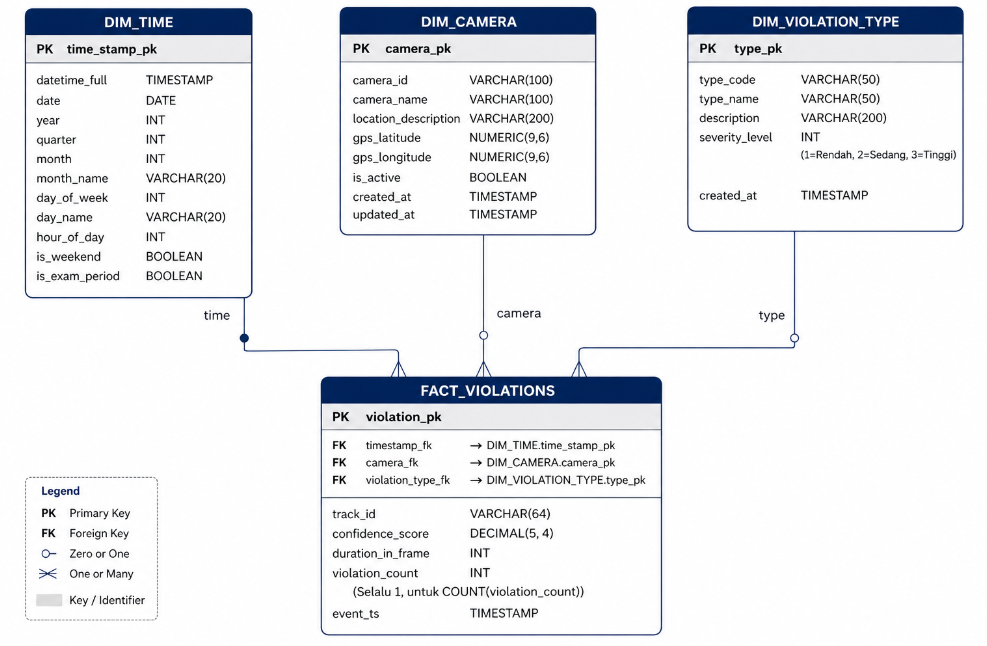
\includegraphics[width=1\textwidth]{gambar/star_schema_helm.png}
\caption{Desain Skema Bintang Data Mart Pelanggaran Helm}
\label{fig:stardesign}
\end{figure}

\section{Rancangan Dashboard Analitik}
Visualisasi hasil deteksi dan pelacakan dirancang dengan \textit{Grafana} yang terhubung ke \textit{data mart} untuk menyajikan ringkasan operasional dan historis secara cepat. Dashboard memuat indikator utama seperti total pelanggaran, jam tersibuk, dan rata-rata jeda antar-pelanggaran, serta analisis tren melalui grafik deret waktu 15 menit, akumulasi harian, dan komposisi periode pagi, siang, dan sore. Selain itu, dashboard juga menampilkan performa sistem dan model melalui distribusi tingkat keyakinan deteksi dan latensi pemrosesan, serta analisis strategis berupa peta panas temporal dan tabel agregat seperti \textit{Top 5 Jam Tersibuk} untuk mendukung pemantauan dan pengambilan keputusan secara lebih efisien.

\section{Alur Penelitian}
\label{sec:alur_penelitian}
Alur penelitian terdiri atas empat tahap utama, mulai dari persiapan data hingga evaluasi sistem (Gambar~\ref{fig:flow-research-systematic}).

\subsection{Tahap 1: Persiapan dan Pra-pemrosesan Data}
Tahap ini menyiapkan dataset dan lingkungan eksperimen untuk pelatihan model visi komputer.
\begin{enumerate}[a.]
\item {Pengumpulan rekaman dan ekstraksi frame selektif}: data primer diperoleh dari rekaman video luring CCTV di gerbang utama Itera. \textit{Frame} diekstraksi secara selektif berdasarkan kualitas visual untuk membentuk \textit{ITERA Helmet Dataset}.
\item {Anotasi objek dan analisis distribusi kelas}: anotasi manual \textit{bounding box} dilakukan pada tiga kelas, yaitu \texttt{DRIVER\_HELMET}, \texttt{DRIVER\_NO\_HELMET}, dan \texttt{MOTORCYCLE}. Distribusi kelas dianalisis untuk mengurangi potensi bias pelatihan.
\item {Pra-pemrosesan dan augmentasi data}: citra distandarkan ke resolusi $640 \times 640$ piksel. Augmentasi geometris dan fotometrik (rotasi, \textit{shear}, eksposur, \textit{noise}, dan \textit{motion blur}) diterapkan untuk meningkatkan generalisasi model.
\end{enumerate}

\subsection{Tahap 2: Pengembangan Model Visi Komputer}
Tahap ini berfokus pada pelatihan dan evaluasi model deteksi objek untuk mengenali atribut keselamatan berkendara.
\begin{enumerate}[a.]
\item {Pelatihan model YOLOv8}: model dilatih selama 300 \textit{epoch} dengan penalaan hiperparameter. Proses pelatihan dipantau melalui \textit{box loss}, \textit{class loss}, dan \textit{distribution focal loss} untuk memastikan konvergensi yang stabil.
\item {Evaluasi kinerja model}: performa model dievaluasi menggunakan mAP@50, \textit{precision}, dan \textit{recall}, baik secara agregat maupun per kelas.
\end{enumerate}

\subsection{Tahap 3: Konstruksi Pipeline Streaming Real-Time}
Tahap ini membangun pipeline streaming terdistribusi untuk mengubah deteksi mentah menjadi \textit{event} terverifikasi.
\begin{enumerate}[a.]
\item {Integrasi inferensi dan pelacakan}: inferensi YOLOv8 diintegrasikan dengan pelacakan multiobjek ByteTrack pada sisi \textit{edge} untuk menjaga identitas kendaraan (\textit{Track ID}) secara persisten.
\item {Penerapan filter logika bertingkat}: metrik IoA digunakan untuk memvalidasi asosiasi antara pengendara dan sepeda motor, lalu konfirmasi temporal \textit{N-frame} diterapkan untuk menekan \textit{false positive} akibat oklusi sesaat.
\item {Serialisasi dan transmisi pesan}: data anomali yang lolos validasi dikemas dalam \textit{payload} JSON dan dikirim melalui Apache Kafka dengan kunci partisi \texttt{camera\_id:track\_id} agar domain urutan kejadian tetap konsisten per kamera.
\item {Pemrosesan ETL streaming}: Apache Spark Structured Streaming mengonsumsi \textit{event} dari Kafka, melakukan \textit{micro-batching}, deduplikasi berbasis \texttt{event\_id} dengan watermark 30 detik, serta ekstraksi dimensi waktu sebelum pemuatan idempotent ke PostgreSQL melalui mekanisme \textit{upsert}.
\item {Evaluasi kinerja pipeline}: efisiensi sistem diukur melalui \textit{throughput} (\textit{frame} per detik) dan latensi pemrosesan pada setiap subsistem.
\end{enumerate}

\subsection{Tahap 4: Implementasi Data Mart dan Visualisasi}
Tahap terakhir mengonsolidasikan data operasional ke \textit{data mart} analitik dan mengevaluasi fungsionalitas akhir sistem.
\begin{enumerate}[a.]
\item {Pemuatan data ke skema bintang}: data dimuat ke PostgreSQL dengan desain \textit{star schema}. Skema ini memisahkan tabel fakta (\texttt{fact\_violations}) dan tabel dimensi (\texttt{dim\_camera}, \texttt{dim\_time}, \texttt{dim\_violation\_type}) untuk mempercepat kueri agregasi.
\item {Visualisasi dasbor analitik}: antarmuka pemantauan dibangun di Grafana yang terhubung langsung ke \textit{data mart} untuk menyajikan metrik operasional secara interaktif.
\end{enumerate}

\begin{figure}[p]
\centering
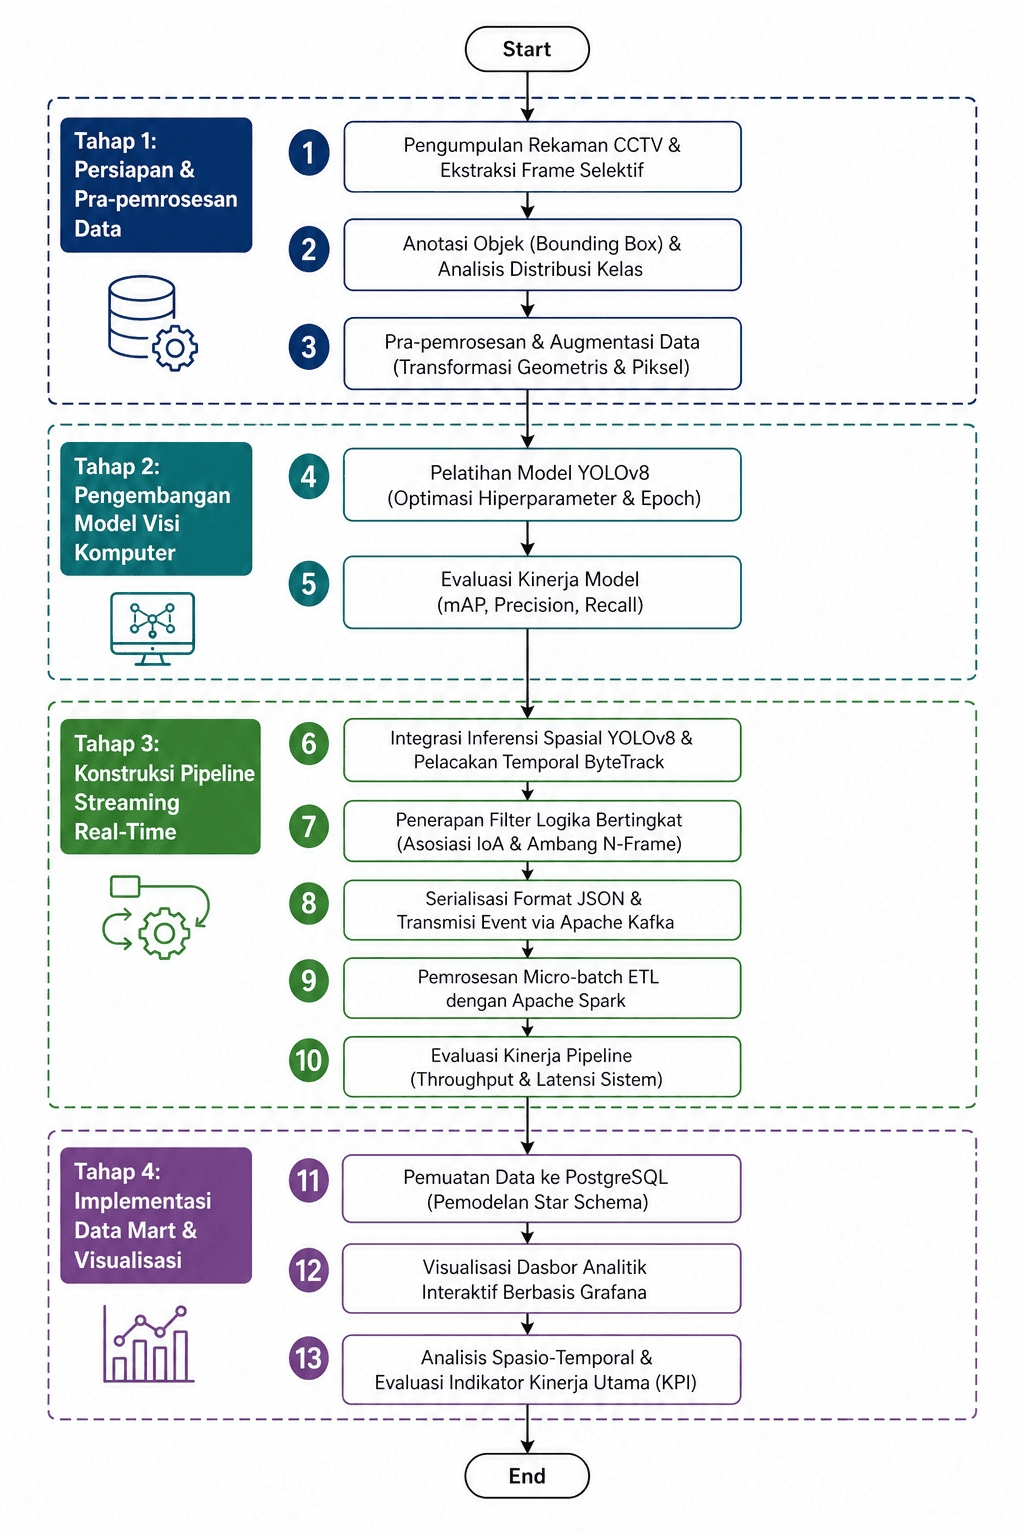
\includegraphics[width=0.8\textwidth,height=0.78\textheight,keepaspectratio]{gambar/alur penelitian.png}
\caption{Diagram Alur Penelitian Sistem Pelacakan Pelanggaran Helm}
\label{fig:flow-research-systematic}
\end{figure}


% % Bab 4 hasil dan pembahasan
% ============================================================
% BAB IV — HASIL DAN PEMBAHASAN
% ITERA Smart Sentinel: Sistem Deteksi & Analitik Pelanggaran Helm Real-time
% ============================================================

\chapter{HASIL DAN PEMBAHASAN}
\label{chap:hasil}

% ============================================================
\section{Pengembangan Model Deteksi Helm Berbasis YOLOv8}
\label{sec:model-deteksi}
Subbab ini menguraikan pengembangan model deteksi YOLOv8 untuk atribut keselamatan berkendara di area gerbang kampus. Pembahasan menyusur empat tahap: analisis dataset, pra-pemrosesan dan augmentasi, dinamika pelatihan, serta evaluasi kinerja sebelum model diintegrasikan ke \textit{pipeline} pemrosesan video waktu nyata.
% ------------------------------------------------------------
\subsection{Eksplorasi Data dan Analisis Distribusi Objek}
\label{subsec:eda-dataset}
% ------------------------------------------------------------

Analisis eksploratif dilakukan pada dataset mentah hasil tangkapan CCTV. Dataset memuat 390 citra unik berukuran median $1280 \times 720$ piksel dengan total 2.369 anotasi objek atau rata-rata 6,1 anotasi per citra. Tabel~\ref{tab:distribusi-objek} merinci distribusi anotasi pada setiap kelas.

\begin{table}[htbp]
  \centering
  \caption{Distribusi anotasi objek pada dataset awal.}
  \label{tab:distribusi-objek}
  \begin{tabular}{clc}
    \hline
    \textbf{ID objek} & \textbf{Nama Objek} & \textbf{Jumlah Anotasi} \\
    \hline
    0 & \texttt{DRIVER\_HELMET}     & 730 \\
    1 & \texttt{DRIVER\_NO\_HELMET} & 718 \\
    2 & \texttt{MOTORCYCLE}         & 921 \\
    \hline
    \textbf{Total} & & \textbf{2.369} \\
    \hline
  \end{tabular}
\end{table}

Tabel~\ref{tab:distribusi-objek} memusatkan perhatian pada dua kelas pelanggaran yang menjadi target utama penelitian, yaitu \texttt{DRIVER\_HELMET} dengan 730 anotasi dan \texttt{DRIVER\_NO\_HELMET} dengan 718 anotasi. Selisih keduanya hanya 12 anotasi atau rasio 1{,}02:1, sehingga jumlahnya bisa dianggap setara. Kesetaraan ini penting karena justru kedua kelas itulah yang harus dibedakan model untuk menentukan status pelanggaran; jumlah yang seimbang membuat model tidak berat sebelah ke salah satu kategori. Kelas \texttt{MOTORCYCLE} memiliki 921 anotasi, sekitar 191 sampai 203 lebih banyak daripada dua kelas pelanggaran. Selisih tersebut wajar karena \texttt{MOTORCYCLE} berperan sebagai kelas konteks: badan motor terlihat utuh hampir di setiap citra, sedangkan kepala pengendara kerap tertutup sebagian oleh kaca depan atau penumpang sehingga anotasi pengendara tidak sebanyak anotasi motor.

Suatu dataset mulai dikategorikan mengalami \textit{class imbalance} apabila nilai \textit{imbalance ratio} (IR) melebihi 1,5:1\cite{kraiem2021resampling}. Pada penelitian ini, rasio kelas mayoritas (\texttt{MOTORCYCLE}) terhadap kelas minoritas (\texttt{DRIVER\_NO\_HELMET}) bernilai 921:718 atau 1,28:1, masih di bawah ambang tersebut. Distribusi ketiga kelas dengan demikian tergolong seimbang dan risiko bias model ke kelas mayoritas tergolong rendah.

Selain dari sisi jumlah, kualitas dataset juga dilihat dari posisi kemunculan objek pada bidang pandang kamera. Gambar~\ref{fig:heatmap-per-class} menyajikan peta panas anotasi dengan gradasi biru muda hingga merah pekat untuk menggambarkan kepadatan \textit{bounding box} di setiap \textit{grid} citra. Pada legenda peta panas, nilai minimum, kuartil pertama, dan median sama-sama 0 anotasi, kuartil ketiga 11 anotasi, sedangkan \textit{grid} terpadat memuat 172 anotasi. Angka tersebut menandakan bahwa anotasi terpusat di sebagian kecil area, sementara sebagian besar \textit{grid} citra kosong.

\begin{figure}[htbp]
  \centering
  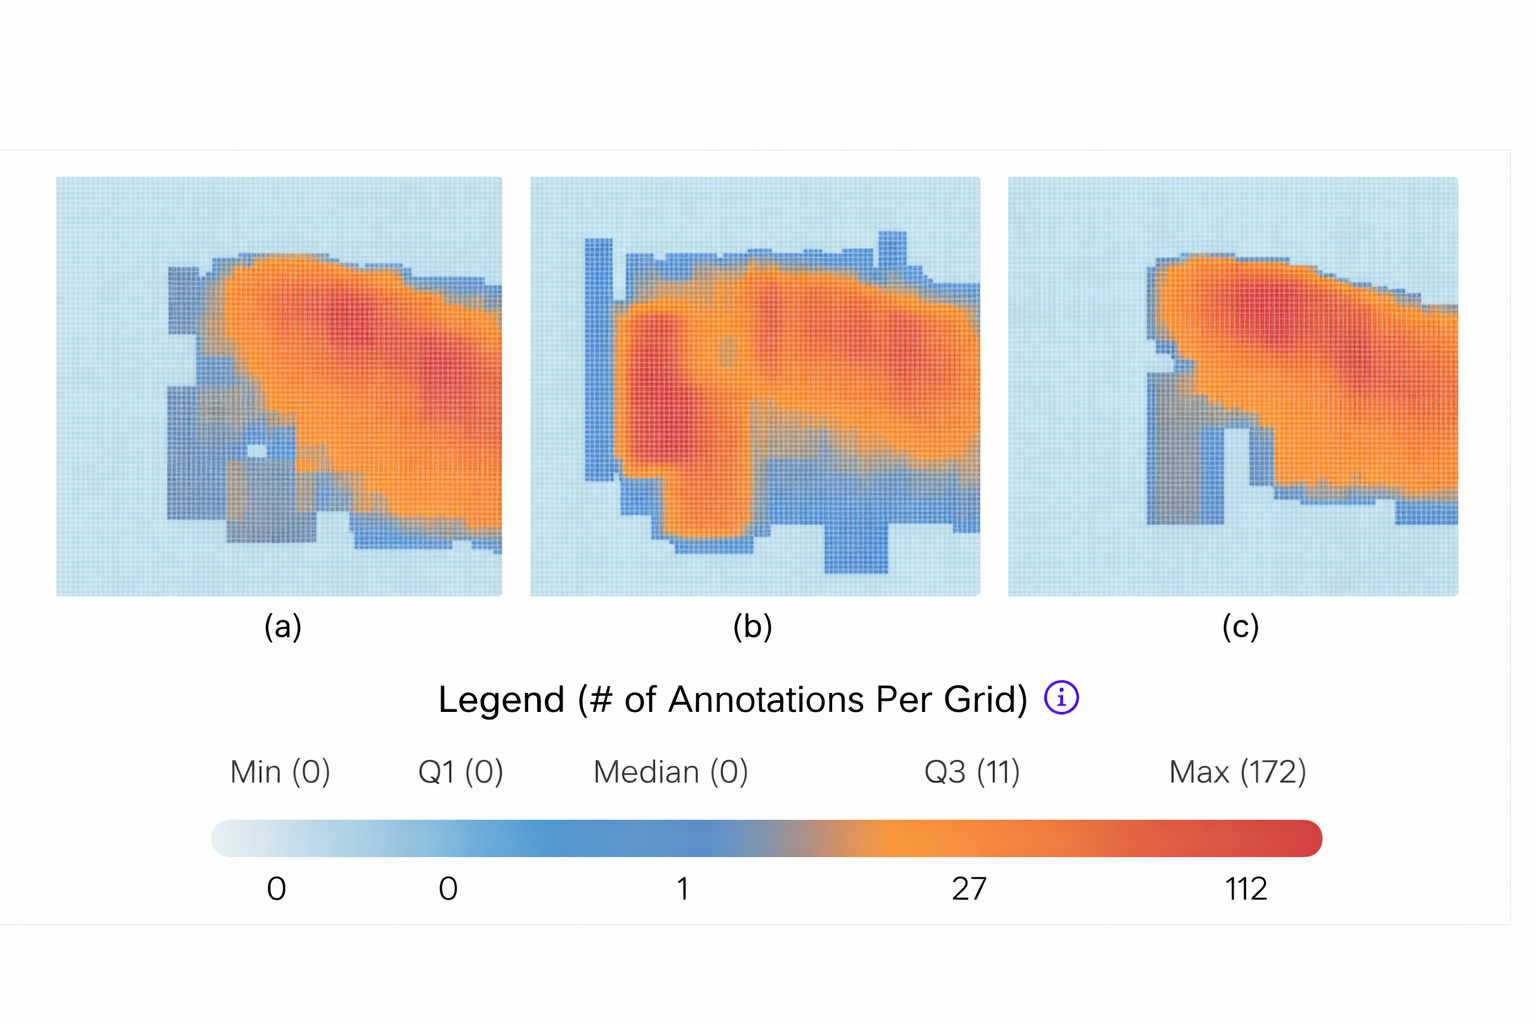
\includegraphics[width=0.95\textwidth]{gambar/heatmap_anotation_class.png}
\caption{Peta panas anotasi (\textit{annotation heatmap}) spasial berdasarkan objek: a) \texttt{DRIVER\_HELMET}, b) \texttt{DRIVER\_NO\_HELMET}, dan c) \texttt{MOTORCYCLE}.}
\label{fig:heatmap-per-class}
\end{figure}

Pada Gambar~\ref{fig:heatmap-per-class}(a), anotasi kelas \texttt{DRIVER\_HELMET} mengumpul di bagian tengah hingga kanan atas citra dengan titik paling padat tepat di lajur masuk utama. Pola sebaran kelas \texttt{DRIVER\_NO\_HELMET} pada Gambar~\ref{fig:heatmap-per-class}(b) hampir sama, hanya saja zona terpadatnya sedikit bergeser ke arah kiri tengah; pergeseran ini mencerminkan kebiasaan sebagian pengendara mengambil sisi tertentu saat masuk gerbang. Gambar~\ref{fig:heatmap-per-class}(c) untuk kelas \texttt{MOTORCYCLE} memiliki zona kepadatan yang nyaris sama persis dengan kelas \texttt{DRIVER\_HELMET}, sebab badan motor selalu menyertai pengendara sebagai konteks anotasi. Karena ketiga kelas terpusat pada wilayah yang relatif sama, \textit{Region of Interest} (ROI) ditarik mengikuti kontur jalan dan kira-kira mencakup bagian tengah sampai kanan atas citra.

Di luar ROI, warna peta panas didominasi biru muda hingga abu-abu yang berarti \textit{grid} di area tersebut hampir tidak memuat anotasi. Wilayah ini mencakup langit di bagian atas, trotoar, dan jalur berlawanan di tepi citra; kendaraan dan pengendara tidak melintas di sana sehingga tidak ada \textit{bounding box} yang muncul. Dengan membatasi inferensi pada ROI, area latar yang kosong tidak ikut diproses dan YOLOv8 hanya bekerja di zona yang memang aktif dilewati kendaraan. Cara ini mengurangi beban komputasi sekaligus menaikkan \textit{precision} dan menekan \textit{false positive} saat inferensi waktu nyata.

% ------------------------------------------------------------
% ------------------------------------------------------------
\subsection{Pra-pemrosesan dan Strategi Augmentasi Data}
\label{subsec:preprocessing-augmentasi}
% ------------------------------------------------------------

Pra-pemrosesan dan augmentasi mengubah 390 citra mentah menjadi 856 sampel pelatihan terstandarisasi. Setiap citra dikalibrasi dengan \textit{auto-orient}, lalu diubah ukurannya (\textit{resize}) ke resolusi seragam $640 \times 640$ piksel. Tahap augmentasi kemudian menghasilkan tiga variasi sintetis untuk setiap citra asli, dengan rincian hiperparameter pada Tabel~\ref{tab:augmentasi}.

Pemilihan resolusi $640 \times 640$ piksel pada YOLOv8n didasari tiga pertimbangan teknis. Pertama, \textit{backbone} YOLOv8 memakai \textit{stride} maksimum 32 sehingga ukuran masukan harus kelipatan 32 agar peta fitur pada level deteksi P3, P4, dan P5 berdimensi bilangan bulat tanpa \textit{padding} tambahan; nilai 640 memenuhi syarat tersebut karena $640 \div 32 = 20$. Kedua, $640 \times 640$ adalah resolusi standar saat YOLOv8 dilatih pada dataset COCO, sehingga bobot pra-latih dapat dipakai langsung dan kalibrasi \textit{head} deteksi tidak perlu disesuaikan ulang. Ketiga, varian ringan YOLOv8 --- termasuk YOLOv8n yang dipakai pada penelitian ini --- dirancang untuk inferensi waktu nyata pada perangkat tepi; resolusi $640 \times 640$ menjaga keseimbangan antara akurasi deteksi objek kecil seperti helm dan beban komputasi yang masih realistis untuk pemrosesan \textit{streaming} CCTV. Resolusi yang lebih besar seperti $1280 \times 1280$ memang menaikkan akurasi tetapi memperberat inferensi, sedangkan resolusi yang lebih kecil seperti $320 \times 320$ membuat detail kepala pengendara hilang karena hanya tertangkap beberapa piksel.

Strategi augmentasi disusun untuk mereplikasi gangguan visual yang lazim terjadi pada kamera pengawas luar ruang. Setiap teknik divisualisasikan dengan citra sebelum dan sesudah augmentasi pada Gambar~\ref{fig:aug-rotasi} sampai Gambar~\ref{fig:aug-noise}, sedangkan parameter \textit{motion blur} dirinci pada Tabel~\ref{tab:augmentasi}.

\begin{figure}[H]
  \centering
  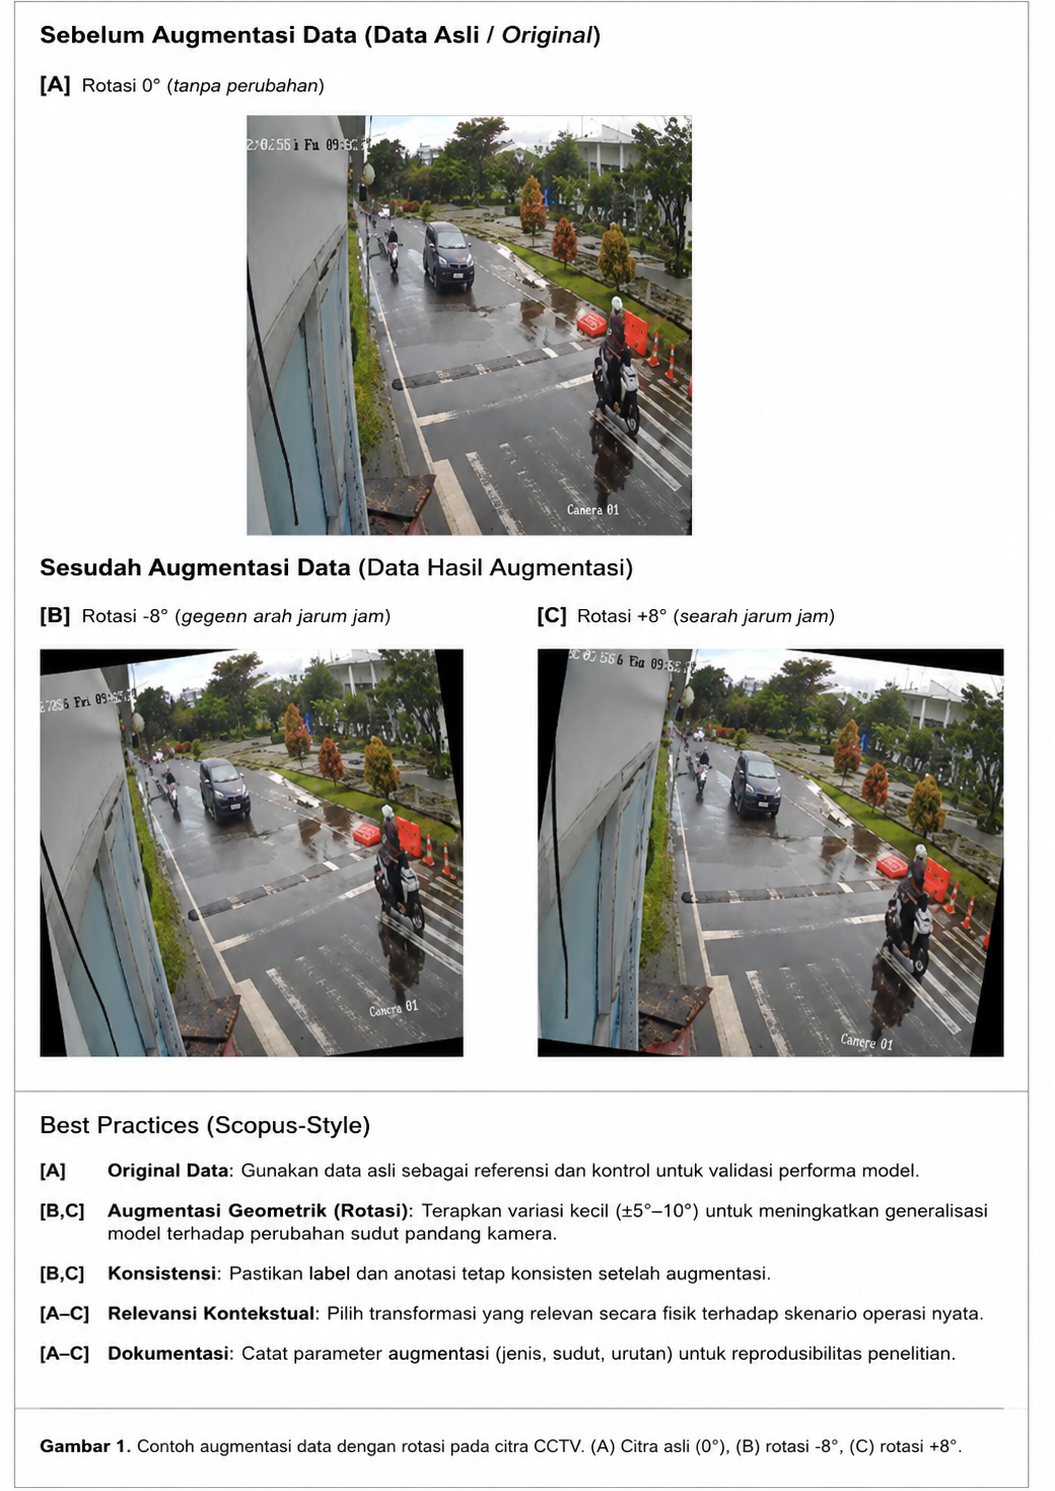
\includegraphics[width=0.85\textwidth]{gambar/aug_rotasi.png}
  \caption{Augmentasi rotasi pada rentang $-8^\circ$ sampai $+8^\circ$.}
  \label{fig:aug-rotasi}
\end{figure}

Augmentasi rotasi memutar citra dalam rentang $-8^\circ$ sampai $+8^\circ$ untuk meniru pergeseran sudut tiang kamera akibat getaran atau dorongan angin. Kamera CCTV pada tiang sering kali sedikit miring dari posisi awal sehingga horizon citra ikut berubah. Pelatihan menggunakan citra hasil rotasi membuat model tidak bergantung pada orientasi horizon yang sempurna ketika mengenali pengendara dan motor.

\begin{figure}[H]
  \centering
  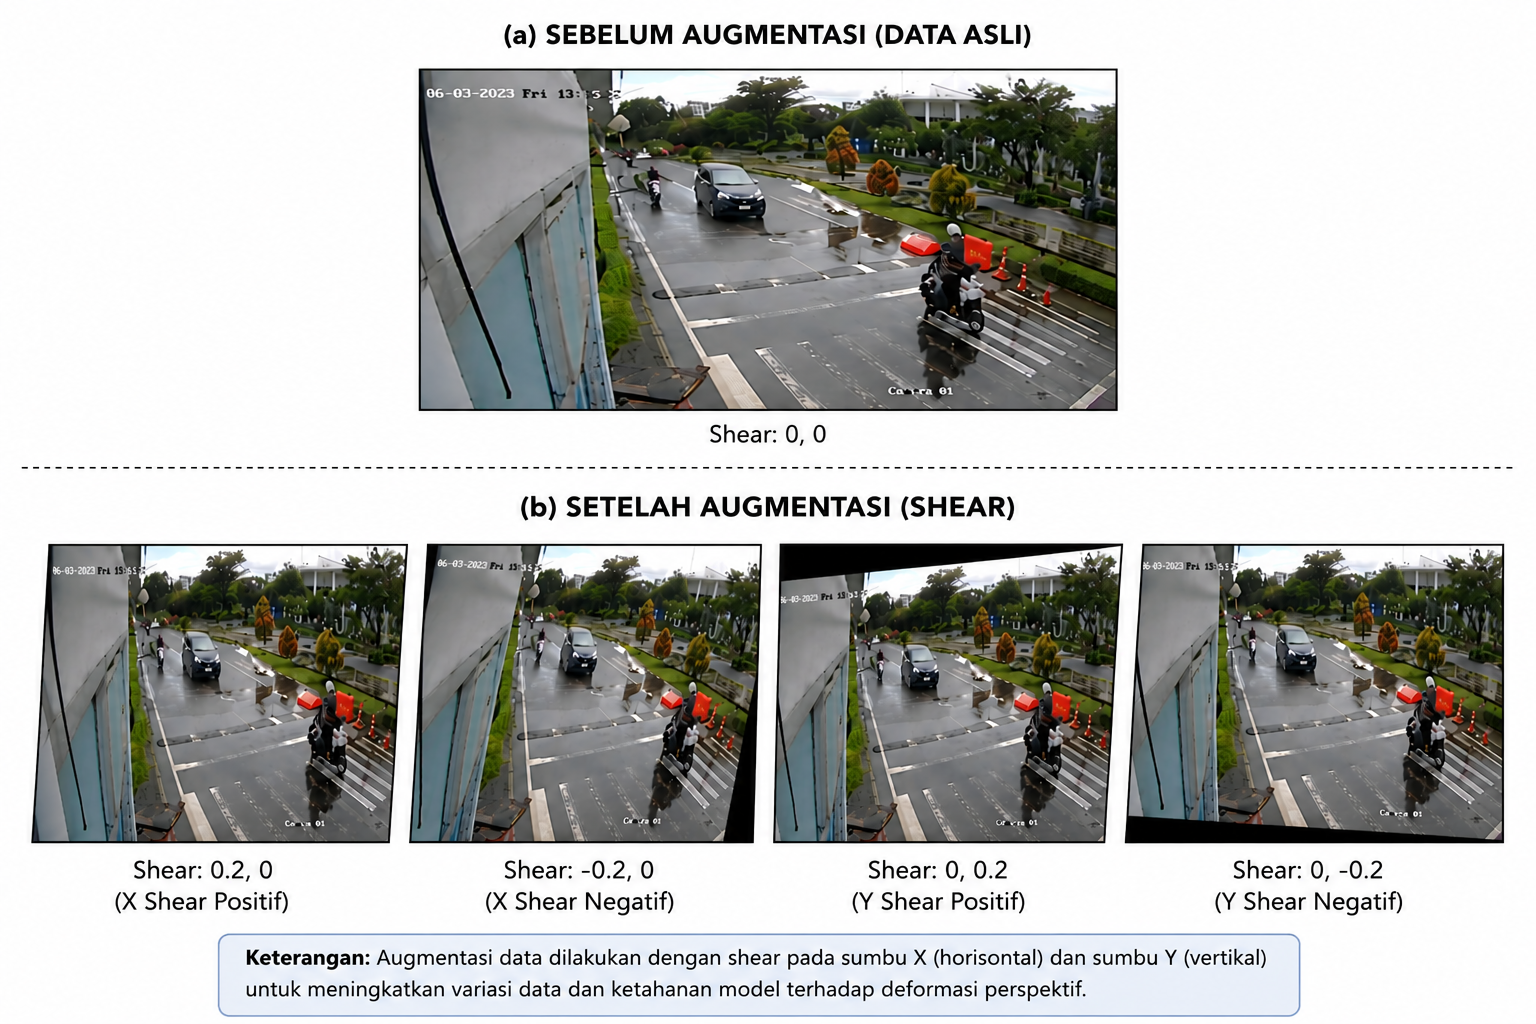
\includegraphics[width=0.95\textwidth]{gambar/aug_shear.png}
  \caption{Augmentasi \textit{shear} pada sumbu X dan Y dengan nilai $\pm 0{,}2$.}
  \label{fig:aug-shear}
\end{figure}

Augmentasi \textit{shear} memiringkan citra pada sumbu X dan Y sebesar $\pm 0{,}2$ untuk meniru distorsi perspektif ketika kamera tidak tegak lurus dengan bidang jalan. Empat varian (X positif, X negatif, Y positif, Y negatif) memperluas variasi sudut pandang sehingga model lebih tahan saat sudut pandang kamera di lapangan berbeda dari sudut pelatihan.

\begin{figure}[H]
  \centering
  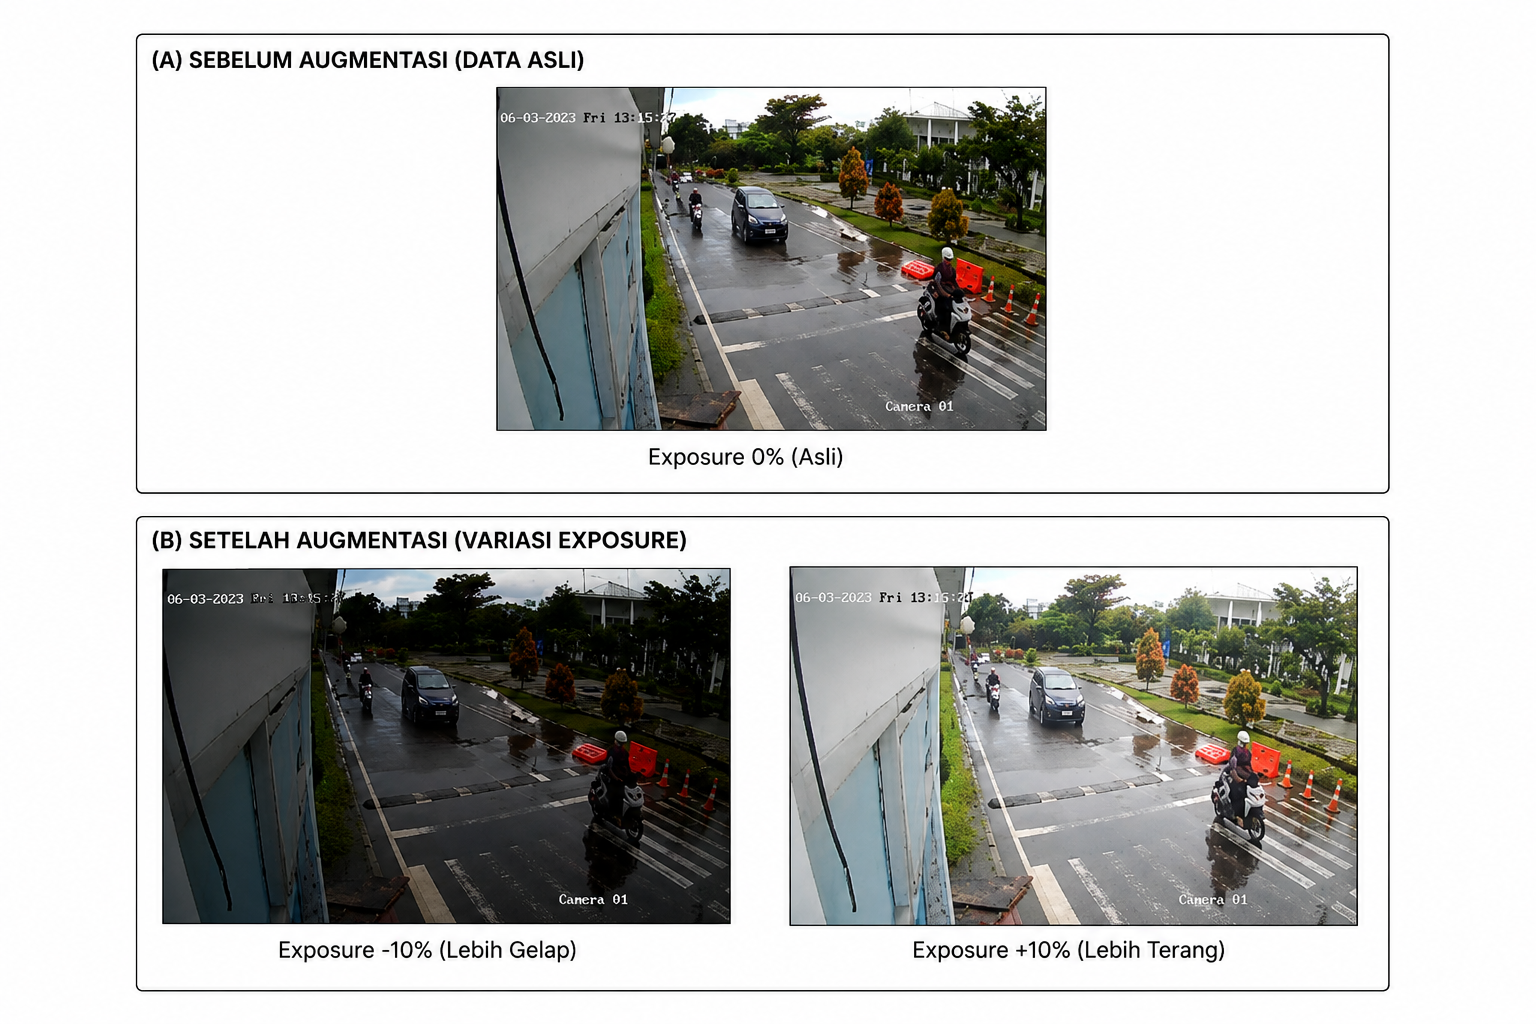
\includegraphics[width=0.95\textwidth]{gambar/aug_exposure.png}
  \caption{Augmentasi \textit{exposure} pada rentang $-10\%$ sampai $+10\%$.}
  \label{fig:aug-exposure}
\end{figure}

Variasi \textit{exposure} sebesar $\pm 10\%$ menyimulasikan perubahan iluminasi sepanjang hari, dari pagi yang masih gelap sampai siang yang sangat terang. Citra dengan eksposur $-10\%$ terlihat lebih gelap dengan bayangan yang dominan, sedangkan eksposur $+10\%$ membuat citra lebih cerah dan kontras tampak menurun. Variasi ini menekan ketergantungan model pada nilai kecerahan tertentu sehingga deteksi tetap stabil di berbagai kondisi pencahayaan.

\begin{figure}[H]
  \centering
  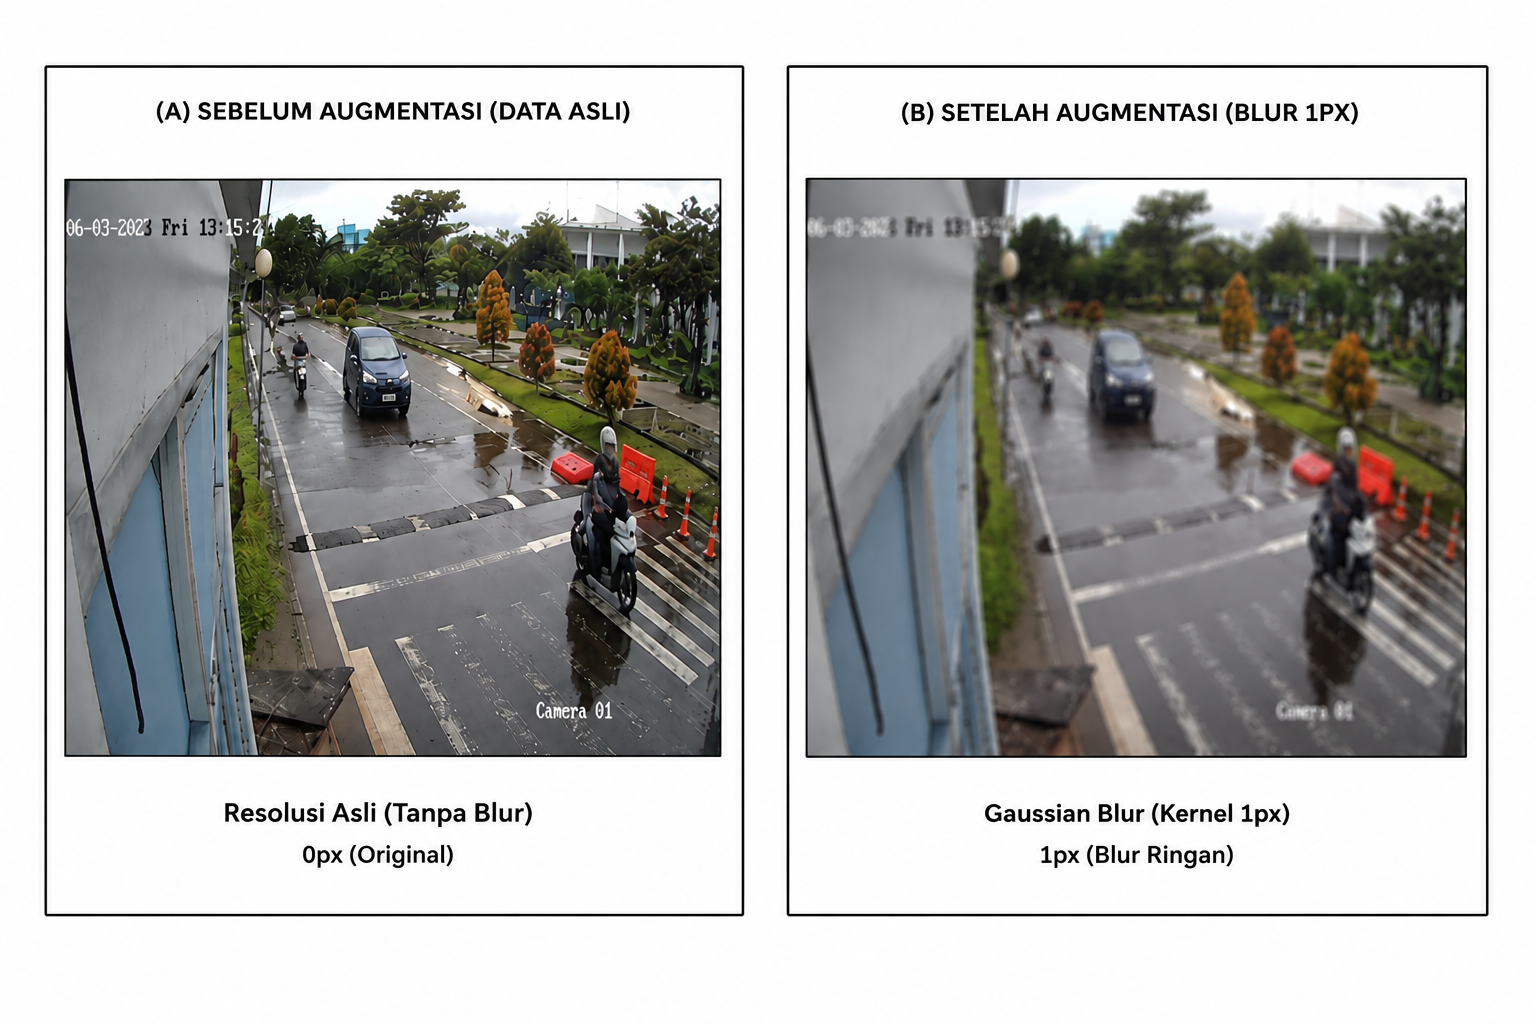
\includegraphics[width=0.95\textwidth]{gambar/aug_blur.png}
  \caption{Augmentasi \textit{Gaussian blur} dengan \textit{kernel} 1 piksel.}
  \label{fig:aug-blur}
\end{figure}

\textit{Gaussian blur} dengan \textit{kernel} 1 piksel meniru kondisi kamera CCTV yang sedikit kehilangan fokus, misalnya karena embun pada lensa atau udara berkabut. Citra hasil augmentasi terlihat sedikit kabur tetapi bentuk objek tetap dapat dibedakan. Augmentasi ini melatih model untuk tidak terlalu bergantung pada ketajaman tepi objek saat melakukan deteksi.

\begin{figure}[H]
  \centering
  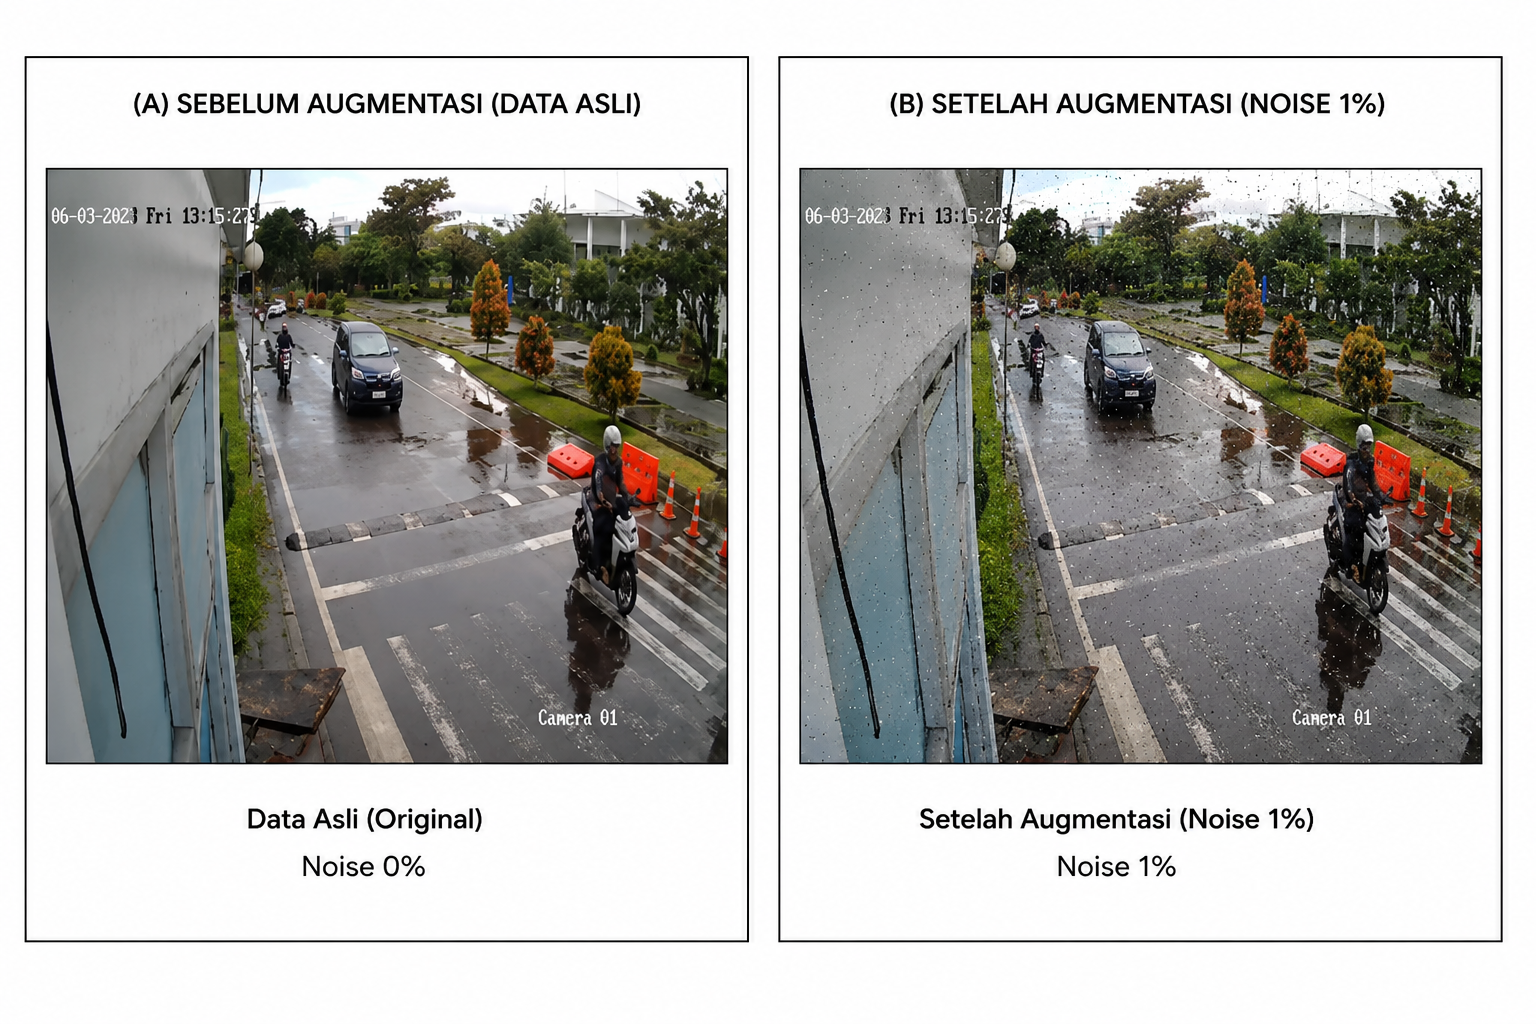
\includegraphics[width=0.95\textwidth]{gambar/aug_noise.png}
  \caption{Augmentasi \textit{additive noise} sebesar 1\% dari total piksel.}
  \label{fig:aug-noise}
\end{figure}

Penambahan \textit{additive noise} sebesar 1\% mereplikasi \textit{grain} sensor kamera pada kondisi cahaya rendah, kompresi \textit{streaming} yang agresif, atau interferensi sinyal pada CCTV analog. Bintik halus yang muncul mengaburkan detail tepi objek tanpa mengubah bentuk keseluruhan, sehingga model tetap dapat mengenali pengendara meskipun citra penuh artefak.

Kelima teknik di atas dilengkapi dengan \textit{motion blur} berpanjang 10 piksel yang meniru jejak gerak ketika kendaraan melintas cepat atau \textit{frame rate} CCTV menurun. Secara keseluruhan, kombinasi enam teknik tersebut menekan risiko \textit{overfitting} terhadap kondisi visual tertentu dan mendorong model membentuk representasi semantik yang lebih kuat \cite{shorten2019survey}.

% ------------------------------------------------------------
\subsection{Konfigurasi Pemisahan Dataset dan Dinamika Pelatihan}
\label{subsec:training-config}
% ------------------------------------------------------------

Dataset diperluas dibagi dengan rasio 82\% pelatihan (699 citra), 9\% validasi (79 citra), dan 9\% pengujian (78 citra). Pembagian ini memberi paparan data pelatihan yang cukup luas dan tetap menyisakan himpunan terpisah untuk memantau generalisasi selama optimasi. Pelatihan berjalan selama 300 \textit{epoch} dengan memantau tiga komponen galat: \textit{box loss}, \textit{class loss}, dan \textit{distribution focal loss} (DFL). Gambar~\ref{fig:training-graphs} menampilkan dinamika ketiga metrik tersebut.

Pada Gambar~\ref{fig:training-graphs}, kurva pelatihan konvergen dengan stabil. Penurunan konsisten terlihat pada \texttt{train/box\_loss}, \texttt{train/cls\_loss}, dan \texttt{train/dfl\_loss} seiring bertambahnya iterasi. Pada data validasi, dinamika paling jelas terbaca pada \texttt{val/box\_loss} dan \texttt{val/dfl\_loss}. Pada fase awal (0--40 \textit{epoch}), kedua kurva turun tajam saat model mempelajari ciri dasar objek besar seperti sasis \texttt{MOTORCYCLE}.

Pada fase pertengahan (\textit{epoch} 50--150), kurva validasi berfluktuasi dengan beberapa lonjakan. Pola tersebut menandakan generalisasi spasial yang belum stabil. Saat sensitivitas deteksi meningkat, model ikut memprediksi objek sekunder di luar \textit{Region of Interest} (ROI), misalnya tekstur latar yang menyerupai helm atau motor, sehingga \textit{false positive} dan galat ikut naik. Pola serupa dilaporkan pada studi yang menyoroti efek ketidakseimbangan data dan variasi skala terhadap stabilitas deteksi pra-konvergensi \cite{oksuz2020imbalance}. Pembaruan bobot lanjutan meredakan fluktuasi pada sepertiga akhir pelatihan (mendekati 300 \textit{epoch}); kurva validasi kembali stabil tanpa gejala \textit{overfitting}. Pada titik ini, model YOLOv8 telah menjepit batas spasial lajur kendaraan dengan lebih tegas dan mengurangi respons terhadap anomali di luar area jalan.

\begin{figure}[H]
\centering
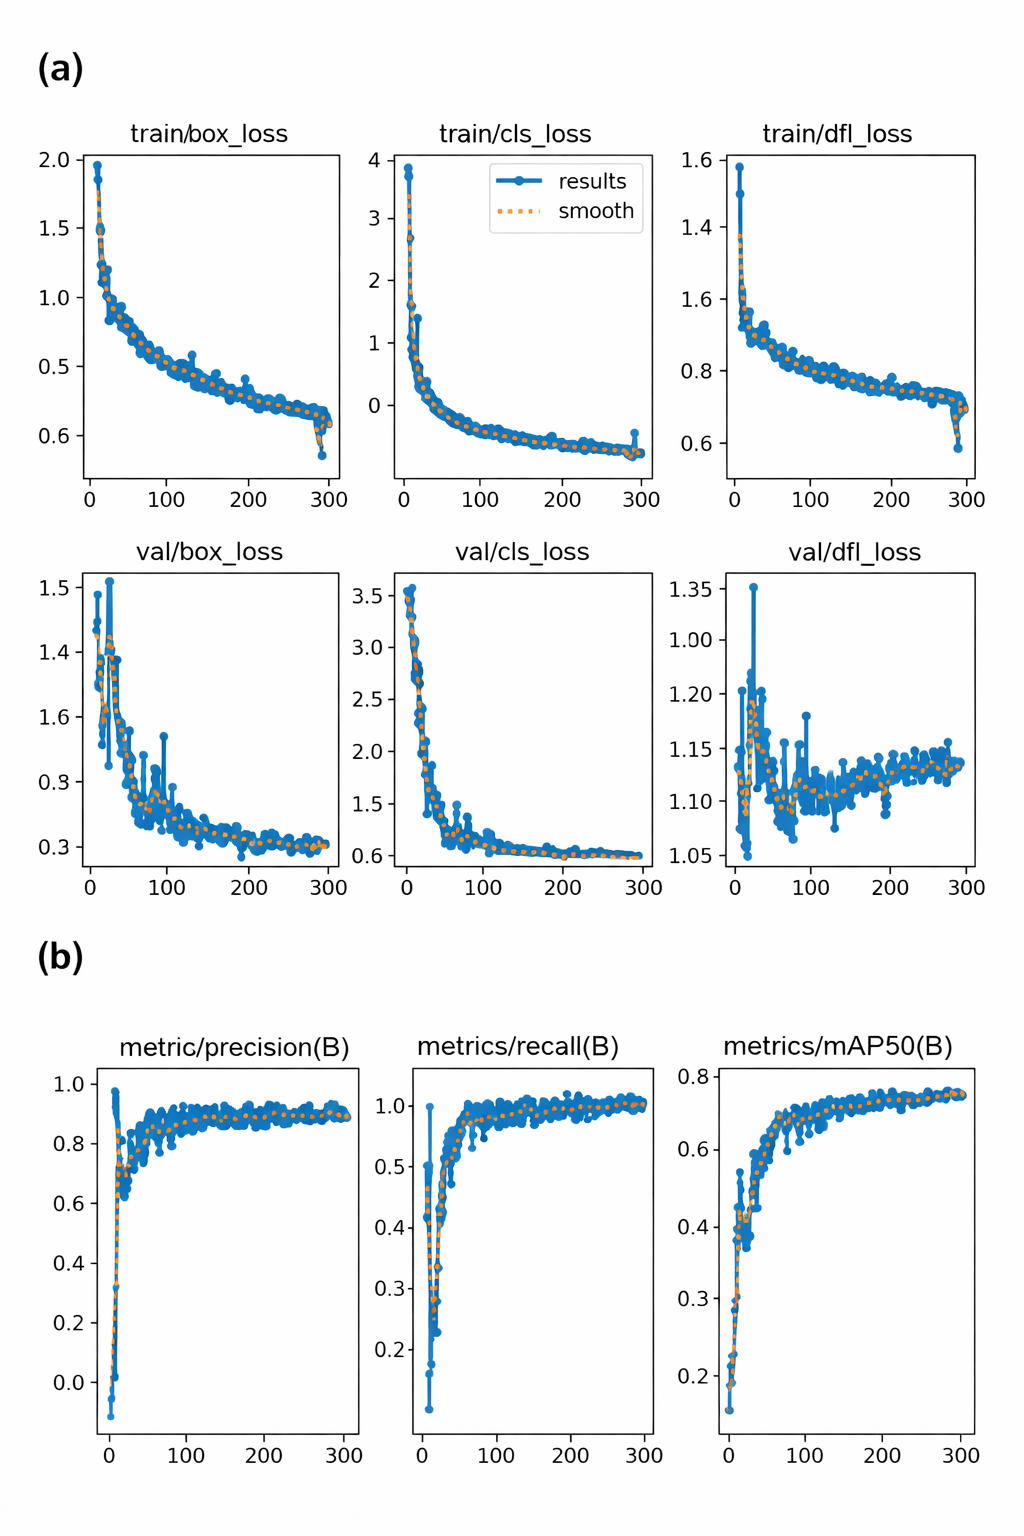
\includegraphics[width=\textwidth,height=0.6\textheight,keepaspectratio]{gambar/log_traning_model.png}
\caption{Kurva pelatihan dan validasi model YOLOv8 selama 300 \textit{epoch}, mencakup \textit{box loss}, \textit{class loss}, \textit{DFL}, serta metrik \textit{precision}, \textit{recall}, dan mAP.}
\label{fig:training-graphs}
\end{figure}

\subsection{Evaluasi Kuantitatif dan Analisis Kinerja Model Deteksi}
\label{subsec:evaluasi-kinerja}
% ============================================================

Evaluasi agregat dilakukan pada himpunan data validasi (\textit{validation set}) menggunakan metrik standar visi komputer. Hasil agregat tersebut disajikan pada Tabel~\ref{tab:metrik-validasi}.

% --- EVIDENCE 1 ---
\begin{table}[htbp]
\centering
\caption{Kinerja agregat model YOLOv8 pada himpunan data validasi.}
\label{tab:metrik-validasi}
\begin{tabular}{lc}
\toprule
\textbf{Metrik Evaluasi} & \textbf{Pencapaian} \\
\midrule
\textit{Mean Average Precision} (mAP@50) & 91,4\% \\
\textit{Precision}  & 87,5\% \\
\textit{Recall}     & 86,5\% \\
\bottomrule
\end{tabular}
\end{table}

% --- ANALITIK 1 ---
Pada Tabel~\ref{tab:metrik-validasi}, \textit{precision} (87,5\%) dan \textit{recall} (86,5\%) hanya berselisih 1,0 poin, sehingga model tidak agresif dan tidak konservatif dalam mendeteksi objek. Skor F1 gabungan berada di kisaran 87,0\%, mengindikasikan klasifikasi dan lokalisasi yang seimbang. Kinerja ini juga didukung oleh pemanfaatan \textit{Region of Interest} (ROI). Pembatasan area deteksi via ROI mengurangi gangguan latar dan menekan deteksi positif palsu (\textit{false positives}), sehingga \textit{precision} tetap di atas 85\%. Dalam konteks operasional, ambang \textit{precision} di atas 85\% diperlukan untuk menurunkan frekuensi alarm palsu pada gudang analitik \textit{streaming}.

Nilai \textit{Mean Average Precision} (mAP@50) 91,4\% kompetitif dengan studi deteksi pelanggaran helm berbasis YOLOv8 pada skenario waktu nyata \cite{aboah2023helmet}. Meskipun demikian, \textit{precision} dan \textit{recall} yang masih di bawah 90\% menyiratkan kelemahan model pada objek kecil dan fitur ambigu. Selisih ukuran \textit{bounding box} antara badan sepeda motor dan area kepala pengendara cukup ekstrem; saat objek menjauh dari kamera, informasi visual area kepala makin terbatas dan model lebih rentan keliru membedakan pengendara berhelm, bertopi, atau berambut tebal. Walau begitu, \textit{recall} 86,5\% mengindikasikan bahwa pelanggaran yang lolos deteksi (\textit{false negatives}) masih dalam jumlah terkendali.

Kemampuan generalisasi model terhadap variasi visual yang belum pernah dilihat dinilai melalui pengujian per objek menggunakan himpunan data uji (\textit{test set}). Rincian metrik \textit{Average Precision} (AP) pada ambang IoU 50\% untuk tiap objek target disajikan pada Tabel~\ref{tab:metrik-test-objek}.

% --- EVIDENCE 2 ---
\begin{table}[htbp]
\centering
\caption{Kinerja \textit{Average Precision} (AP@50) per objek pada himpunan data uji.}
\label{tab:metrik-test-objek}
\begin{tabular}{lc}
\toprule
\textbf{Kategori Objek Target} & \textbf{AP@50} \\
\midrule
\texttt{Keseluruhan (All)}  & 90,0\% \\
\texttt{MOTORCYCLE}         & 94,0\% \\
\texttt{DRIVER\_NO\_HELMET} & 90,0\% \\
\texttt{DRIVER\_HELMET}     & 87,0\% \\
\bottomrule
\end{tabular}
\end{table}

% --- ANALITIK 2 ---
Tabel~\ref{tab:metrik-test-objek} memperlihatkan variasi kinerja antarobjek. \texttt{MOTORCYCLE} mencatat AP tertinggi (94,0\%), wajar karena badan motor menempati piksel dominan dan bentuknya relatif konsisten antar-citra. Sebaliknya, atribut kepala memiliki AP yang lebih rendah; selisih 7,0 poin antara \texttt{MOTORCYCLE} dan \texttt{DRIVER\_HELMET} menempatkan tantangan utama model bukan pada deteksi objek besar melainkan pada klasifikasi atribut berukuran kecil. Pola ini sejalan dengan isu \textit{scale imbalance} pada deteksi objek kecil yang dilaporkan oleh \cite{oksuz2020imbalance}.

Pada atribut pengendara, model lebih presisi mendeteksi \texttt{DRIVER\_NO\_HELMET} (90,0\%) dibandingkan \texttt{DRIVER\_HELMET} (87,0\%). Selisih 3,0 poin tersebut mengindikasikan fitur visual \textit{tidak berhelm} lebih mudah dipelajari ketimbang variasi tampilan helm di lapangan. Keragaman bentuk, warna, dan tekstur helm yang ditambah pantulan cahaya (\textit{glare}) serta oklusi parsial pada lalu lintas padat menurunkan keterlihatan fitur dan memicu kesalahan klasifikasi (\textit{misclassification}).

Secara agregat, mAP@50 sebesar 90,0\% menunjukkan modul visi komputer beroperasi stabil pada data uji. Tingkat akurasi ini cukup untuk diintegrasikan dengan ByteTrack pada purwarupa waktu nyata di Itera. Peningkatan lanjutan dapat difokuskan pada deteksi atribut kepala agar selisih AP antarobjek menyempit.

% ============================================================
\section{Integrasi YOLOv8 dan ByteTrack dalam \textit{Pipeline Streaming} Waktu Nyata}
\label{sec:integrasi-pipeline}
Setelah model ekstraksi fitur spasial divalidasi, langkah berikutnya adalah mengintegrasikannya ke ekosistem pemrosesan aliran video waktu nyata (\textit{real-time video streaming}). Subbab ini menguraikan arsitektur hulu-ke-hilir (\textit{end-to-end}) yang memadukan deteksi YOLOv8 dan pelacakan multiobjek ByteTrack untuk menjaga persistensi identitas kendaraan. Pembahasan mencakup orkestrasi \textit{pipeline}, penerapan penyaring spasial (\textit{Intersection over Area}) dan temporal (N-\textit{frame}) untuk menekan deteksi palsu, serta evaluasi beban komputasi di simpul tepi (\textit{edge throughput} dan latensi). Bagian akhir mengevaluasi performa distribusi data dengan Apache Kafka dan orkestrasi \textit{micro-batch} Apache Spark untuk memvalidasi ketahanan sistem terhadap lonjakan beban operasional.

\subsection{Arsitektur dan Orkestrasi Pipeline Integrasi}
\label{subsec:pipeline-architecture}
Arsitektur \textit{streaming} memerlukan alur transformasi data yang terstruktur agar informasi mentah berubah menjadi wawasan tanpa beban komputasi berlebih. Bagian ini membedah orkestrasi \textit{pipeline} pada simpul tepi yang membagi proses analitik ke dalam tahapan sekuensial. Penjelasan menyusur perjalanan data: akuisisi matriks piksel, ekstraksi fitur lokalisasi, penetapan identitas objek, penyaringan berbasis aturan (\textit{rule-based filtering}), hingga serialisasi akhir menjadi aliran peristiwa (\textit{event stream}) berformat JSON yang siap ditransmisikan ke pialang pesan (\textit{message broker}).
% ------------------------------------------------------------------
\subsubsection{Diagram Alur Transformasi Data}
\label{subsubsec:pipeline-flowchart}

Pada arsitektur ini, data berubah bertahap di setiap fungsi sistem. Matriks piksel mentah dari kamera pengawas diolah menjadi aliran kejadian melalui ekstraksi fitur, pelacakan identitas, dan validasi berbasis aturan. Alur transformasi tersebut ditampilkan pada Gambar~\ref{fig:pipeline-flow}.

\begin{figure}[htbp]
\centering
\resizebox{\textwidth}{!}{%
\begin{tikzpicture}[
  node distance=0.6cm,
  stage/.style={
    rectangle, rounded corners=4pt, draw=black!70, fill=blue!8,
    minimum width=3.2cm, minimum height=2.6cm, align=center,
    font=\small
  },
  arrow/.style={-{Stealth[length=3mm]}, thick, draw=black!60},
  datalabel/.style={font=\scriptsize\ttfamily, text=black!70, align=center},
]

% Nodes
\node[stage] (input) {
  \textbf{Input Frame}\\[2pt]
  OpenCV
};

\node[stage, right=of input] (yolo) {
  \textbf{YOLOv8}\\[2pt]
  Ekstraksi fitur
};

\node[stage, right=of yolo] (bytrack) {
  \textbf{ByteTrack}\\[2pt]
  Pelacakan multiobjek
};

\node[stage, right=of bytrack] (assoc) {
  \textbf{Asosiasi}\\
  \textbf{spasial}\\[2pt]
  Filter IoA
};

\node[stage, right=of assoc] (violation) {
  \textbf{Logika temporal}\\[2pt]
  Konfirmasi\\
  N-\textit{frame}
};

\node[stage, right=of violation] (kafka) {
  \textbf{Kafka}\\
  \textbf{Producer}\\[2pt]
  Aliran peristiwa
};

% Arrows with data labels
\draw[arrow] (input) -- (yolo)
node[midway, above, datalabel] {}
node[midway, below, datalabel] {};

\draw[arrow] (yolo) -- (bytrack)
node[midway, above, datalabel] {}
node[midway, below, datalabel] {};

\draw[arrow] (bytrack) -- (assoc)
node[midway, above, datalabel] {}
node[midway, below, datalabel] {};

\draw[arrow] (assoc) -- (violation)
node[midway, above, datalabel] {}
node[midway, below, datalabel] {};

\draw[arrow] (violation) -- (kafka)
node[midway, above, datalabel] {}
node[midway, below, datalabel] {};

\end{tikzpicture}
}%
\caption{Diagram alur transformasi data pada \textit{pipeline} pemrosesan tepi. Matriks piksel mentah diolah menjadi fitur spasial, diperkaya dengan identitas temporal, divalidasi, lalu diserialisasi ke format JSON.}
\label{fig:pipeline-flow}
\end{figure}

Pada Gambar~\ref{fig:pipeline-flow}, pemrosesan aliran data langsung memungkinkan analisis video tanpa penyimpanan perantara. Pembagian tugas antara deteksi spasial, pelacakan temporal, dan pengiriman pesan menekan latensi sistem. Pendekatan terdesentralisasi pada simpul tepi ini sejalan dengan praktik \textit{stream processing} latensi rendah pada arsitektur \textit{video analytics} terdistribusi \cite{ayae2017video,kreps2014questioning,cao2017edgeanalytics}.

% ------------------------------------------------------------------
\subsubsection{Tahap 1 \& 2: Akuisisi Citra dan Ekstraksi Fitur Spasial (YOLOv8)}
\label{subsubsec:stage1-2}

Modul akuisisi mengubah \textit{frame} video menjadi matriks numerik BGR berdimensi $1280 \times 720 \times 3$ piksel, lalu menstandarkannya ke $640 \times 640$ piksel. Inferensi YOLOv8 kemudian memetakan matriks tersebut menjadi koordinat \textit{bounding box}, skor keyakinan (\textit{confidence}), dan label objek. Cuplikan hasil ekstraksi fitur spasial pada \textit{frame} awal pengujian disajikan pada Tabel~\ref{tab:output-yolo}.



\begin{table}[htbp]
\centering
\caption{Representasi data \textit{output} inferensi YOLOv8 pada \textit{frame} awal. Volume data menyusut drastis dari jutaan piksel menjadi larik parameter spasial.}
\label{tab:output-yolo}
\footnotesize
\setlength{\tabcolsep}{3pt}
\begin{tabular}{p{1.4cm} p{3.2cm} c c c c c}
\toprule
\textbf{ID Deteksi} & \textbf{Kategori objek} & \textbf{X1} & \textbf{Y1} & \textbf{X2} & \textbf{Y2} & \textbf{Confidence} \\
\midrule
1 & \texttt{MOTORCYCLE}      & 936{,}9  & 374{,}5 & 1061{,}2 & 526{,}2 & 0{,}9398 \\
2 & \texttt{MOTORCYCLE}      & 752{,}5  & 274{,}9 &  828{,}1 & 366{,}3 & 0{,}9262 \\
3 & \texttt{DRIVER\_HELMET}  & 767{,}4  & 227{,}4 &  812{,}6 & 341{,}0 & 0{,}8910 \\
4 & \texttt{DRIVER\_HELMET}  & 970{,}8  & 303{,}9 & 1037{,}8 & 480{,}2 & 0{,}8840 \\
\bottomrule
\end{tabular}
\end{table}

Pada Tabel~\ref{tab:output-yolo}, keluaran YOLOv8 sudah berbentuk representasi spasial ringkas: koordinat \textit{bounding box}, kategori objek, dan skor \textit{confidence}. Pada \textit{frame} awal, dua \texttt{MOTORCYCLE} dan dua \texttt{DRIVER\_HELMET} terdeteksi dengan keyakinan 0{,}8840--0{,}9398. Tingkat keyakinan ini memadai sebagai input untuk tahap pelacakan dan validasi berikutnya.

% ------------------------------------------------------------------
\subsubsection{Tahap 3 \& 4: Pelacakan Multi-Objek dan Asosiasi Spasial (IoA)}
\label{subsubsec:stage3-4}

Pada tahap integrasi, keluaran YOLOv8 yang diproses ByteTrack menghasilkan identitas persisten (\texttt{Track ID}) antar-\textit{frame}. Sistem kemudian menghitung \textit{Intersection over Area} (IoA) untuk memvalidasi relasi fisik antara pengendara dan kendaraan dengan ambang $\geq 0{,}3$. Tabel~\ref{tab:output-bytetrack-ioa} merangkum status validasi asosiasi spasial beserta identitas entitas yang dipertahankan.

Metrik IoA pada Tabel~\ref{tab:output-bytetrack-ioa} mengonfirmasi peran filter spasial dalam mereduksi anomali deteksi. Filter ini memisahkan pengendara aktif dari pejalan kaki di sekitar area lalu lintas. Asosiasi dua tahap pada ByteTrack juga menjaga persistensi identitas saat terjadi oklusi sekaligus mempertahankan stabilitas lokalisasi spasial \cite{zhang2022bytetrack_eccv,ma2023adaptivebytetrack}. Kombinasi ByteTrack dan IoA menekan \textit{false positive} sebelum data diteruskan ke modul penentu jenis pelanggaran.

\begin{table}[htbp]
\centering
\caption{Hasil pemrosesan ByteTrack dan perhitungan IoA. Setiap objek kini memiliki identitas persisten (\textit{Track ID}) dan divalidasi posisi berkendaranya secara spasial.}
\label{tab:output-bytetrack-ioa}
\small
\resizebox{\textwidth}{!}{%
\begin{tabular}{cclcc}
\toprule
\textbf{Track ID} & \textbf{Kategori Objek} & \textbf{Relasi Asosiasi} & \textbf{Skor IoA} & \textbf{Status Validasi} \\
\midrule
1 & \texttt{MOTORCYCLE}      & - & - & Pembawa (\textit{carrier}) \\
2 & \texttt{MOTORCYCLE}      & - & - & Pembawa (\textit{carrier}) \\
3 & \texttt{DRIVER\_HELMET}  & Menunggangi ID 2 & 0{,}5820 & Validasi sukses (\checkmark) \\
4 & \texttt{DRIVER\_HELMET}  & Menunggangi ID 1 & 0{,}5996 & Validasi sukses (\checkmark) \\
\bottomrule
\end{tabular}
}
\end{table}

% ------------------------------------------------------------------
\subsubsection{Tahap 5: Validasi Temporal (N-\textit{frame}) dan Deduplikasi}
\label{subsubsec:stage5}

Logika berbasis aturan menunda klasifikasi pelanggaran instan agar prediksi prematur tidak ikut tercatat. Status \texttt{DRIVER\_NO\_HELMET} hanya dikonfirmasi setelah persisten selama minimal tiga \textit{frame} berturut-turut ($N=3$). Protokol deduplikasi tambahan memastikan satu entitas (\texttt{Track ID}) hanya memicu satu insiden. Dinamika akumulasi konfirmasi temporal ini ditampilkan pada Gambar~\ref{fig:streak-timeline}.

\begin{figure}[htbp]
\centering
\begin{tikzpicture}[
frame/.style={rectangle, draw, minimum width=1.1cm, minimum height=0.7cm,
font=\small, align=center},
confirmed/.style={frame, fill=red!20},
streak/.style={frame, fill=yellow!20},
normal/.style={frame, fill=green!10},
]

% Timeline
\node[normal] (f1) at (0,0) {Frame 1\\streak=1};
\node[streak] (f2) at (2.2,0) {Frame 2\\streak=2};
\node[confirmed] (f3) at (4.4,0) {Frame 3\\streak=3};

% Labels
\node[above=0.3cm of f1, font=\scriptsize] {NO\_HELMET};
\node[above=0.3cm of f2, font=\scriptsize] {NO\_HELMET};
\node[above=0.3cm of f3, font=\scriptsize] {NO\_HELMET};

% Arrow
\draw[-{Stealth}, thick] (f1) -- (f2);
\draw[-{Stealth}, thick] (f2) -- (f3);

% Confirmation marker
\node[below=0.4cm of f3, font=\small\bfseries, text=red!70!black] {%
Ambang $N=3$ Tercapai $\Rightarrow$ Kirim Event
};

% Track ID label
\node[left=0.5cm of f1, font=\small] {\textbf{Track ID = 4:}};

\end{tikzpicture}
\caption{\textit{Timeline} konfirmasi temporal. Pelanggaran hanya dicatat ke \textit{database} apabila model mendeteksi objek tanpa helm secara persisten dalam minimal tiga \textit{frame} berurutan.}
\label{fig:streak-timeline}
\end{figure}

Filter N-\textit{frame} pada Gambar~\ref{fig:streak-timeline} menyaring prediksi yang sempat berubah akibat pantulan cahaya, bayangan, atau gangguan visual singkat, sehingga pencatatan kejadian lebih andal. Deduplikasi per entitas mencegah satu pelanggaran tercatat berulang. Tanpa kedua mekanisme tersebut, satu pengendara tanpa helm yang melintas selama 5 detik pada 15 FPS dapat tercatat hingga 75 kali dan membiaskan ringkasan data pada dasbor.

% ------------------------------------------------------------------
\subsubsection{Tahap 6: Serialisasi Data Kejadian ke Format JSON}
\label{subsubsec:stage6}

Pada tahap akhir simpul tepi, kejadian pelanggaran yang lolos validasi diserialisasi ke format JavaScript Object Notation (JSON). Struktur ringan ini merangkum dimensi spasial, temporal, dan identitas, lalu dipublikasikan ke topik Apache Kafka dengan kompresi Snappy. Format muatan kejadian yang dihasilkan rangkaian pemrosesan disajikan pada Tabel~\ref{tab:json-output}.
\begin{table}[htbp]
\centering
\caption{Struktur muatan data (\textit{JSON event payload}) akhir yang dikirimkan ke Kafka. Data operasional yang dihasilkan kaya dimensi untuk kebutuhan agregasi analitik.}
\label{tab:json-output}
\footnotesize
\setlength{\tabcolsep}{4pt}
\begin{tabular}{p{0.18\textwidth} p{0.24\textwidth} p{0.46\textwidth}}
\toprule
\textbf{Nama Field} & \textbf{Contoh Nilai (Aktual)} & \textbf{Keterangan Dimensi Data} \\
\midrule
\texttt{event\_id}     & \texttt{"b11c5428-0c99..."}    & UUID unik untuk \textit{tracking} insiden \\
\texttt{track\_id}     & \texttt{15}                    & Identitas unik objek dari ByteTrack \\
\texttt{timestamp}     & \texttt{"2026-03-03T20:41..."} & Konteks temporal waktu kejadian \\
\texttt{camera\_id}    & \texttt{"gate\_utama\_01"}     & Konteks lokasi sumber deteksi \\
\texttt{violation\_type} & \texttt{"no\_helmet"}         & Kategori tipe anomali \\
\texttt{confidence}    & \texttt{0.8939}                & Tingkat keyakinan model YOLO (format JSON literal) \\
\texttt{bbox\_[xy12]}  & \texttt{990, 312, 1058, 490}   & Batas spasial (\textit{flattened} untuk \textit{query}) \\
\texttt{frame\_number} & \texttt{3}                     & Posisi kemunculan dalam aliran video \\
\texttt{latency\_ms}   & \texttt{58.94}                 & Metrik performa rangkaian waktu nyata \\
\bottomrule
\end{tabular}
\end{table}
Tabel~\ref{tab:json-output} memperlihatkan bahwa serialisasi mempertahankan seluruh metadata esensial. Kombinasi UUID (\textit{Universally Unique Identifier}) dan stempel waktu (\textit{timestamp}) berpresisi tinggi menjamin ketertelusuran data pada arsitektur hulu-ke-hilir (\textit{end-to-end}). Skema kejadian yang konsisten dan ringkas memungkinkan pialang pesan dan mesin analitik seperti Apache Spark mengonsumsi, mendistribusikan, dan menyimpan aliran data berskala besar pada model pesan terdistribusi yang andal \cite{ayae2017video,kleppmann2017designing}.

% ------------------------------------------------------------------
% \subsubsection{Ringkasan Efisiensi Transformasi Data}
% \label{subsubsec:transformation-summary}

% Sebagai ringkasan, Tabel~\ref{tab:transformation-summary} menunjukkan efisiensi transformasi data pada sistem yang diusulkan.

% \begin{table}[htbp]
% \centering
% \caption{Ringkasan penyusutan ukuran data dan pengayaan informasi dari awal hingga akhir proses.}
% \label{tab:transformation-summary}
% \small
% \begin{tabular}{p{2.8cm}p{3.4cm}p{4.2cm}p{2cm}}
% \toprule
% \textbf{Tahap Pipeline} & \textbf{Tipe Data} & \textbf{Pengayaan Informasi} & \textbf{Ukuran Data} \\
% \midrule
% Akuisisi Frame      & \texttt{Matriks Piksel}    & Piksel lingkungan mentah & $\sim$2.76 MB \\
% YOLOv8 + ByteTrack  & \texttt{sv.Detections}     & BBox, objek, Conf, Track ID & $\sim$1.5 KB \\
% Filter Spasial (IoA)& \texttt{Relasi Matriks}    & Status berkendara motor & $\sim$200 Byte \\
% Filter Temporal     & \texttt{Stateful Counter}  & Eliminasi \textit{False Positive} & (Proses logika) \\
% \textbf{Kafka JSON Stream} & \textbf{\texttt{Format Teks (JSON)}} & \textbf{Event terstruktur utuh} & \textbf{$\sim$350 Byte} \\
% \bottomrule
% \end{tabular}
% \end{table}

% Secara analitis, hasil ini menunjukkan bahwa alur pemrosesan tidak hanya memindahkan data, tetapi juga menyeleksi informasi yang relevan. Data mentah sebesar 2,76 Megabyte berhasil diringkas menjadi catatan terstruktur berukuran sekitar 350 Byte. Rasio penyusutan data yang sangat tinggi (lebih dari $8.000\times$) menunjukkan bahwa kebutuhan lebar pita dari CCTV ke server Kafka tetap ringan bagi infrastruktur kampus. Hasil ini mendukung kelayakan sistem untuk penerapan perangkat terhubung dan \textit{internet of things}.
% ============================================================
\subsection{Evaluasi Stabilitas Pelacakan Multi-Objek (ByteTrack)}
\label{subsec:stabilitas-bytetrack}
% ============================================================

ByteTrack mempertahankan identitas objek (\texttt{Track ID}) secara konsisten sejak kendaraan masuk area pantau hingga keluar jangkauan kamera. Pada pengujian 3.001 \textit{frame} video operasional di gerbang kampus, pelacakan tetap berjalan saat lalu lintas padat. Tabel~\ref{tab:bytetrack-basic-stats} merangkum hasil kuantitatif pelacakan.

\begin{table}[htbp]
\centering
\caption{Statistik beban pelacakan multiobjek oleh algoritma ByteTrack pada video uji (3.001 \textit{frame}).}
\label{tab:bytetrack-basic-stats}
\begin{tabular}{lc}
\toprule
\textbf{Parameter Pelacakan} & \textbf{Hasil} \\
\midrule
Total Objek Unik Terlacak & 134 entitas \\
Rata-rata Objek Aktif per \textit{Frame} & 3,36 objek \\
Puncak Kepadatan Objek Simultan & 11 objek \\
Durasi Pelacakan Terpanjang & 419 \textit{frame} \\
\bottomrule
\end{tabular}
\end{table}

Tabel~\ref{tab:bytetrack-basic-stats} memperlihatkan bahwa pelacakan mencatat 134 objek unik dan tetap stabil pada puncak kepadatan 11 objek per \textit{frame}. Tanpa pelacakan identitas, deteksi per-\textit{frame} pada satu objek yang sama dapat terbaca berulang pada banyak \textit{frame} dan tercatat sebagai banyak pelanggaran. Penerapan \texttt{Track ID} via asosiasi deteksi lintas \textit{frame} memangkas risiko penghitungan berulang dalam satu sesi pelacakan aktif. \texttt{Track ID} pada ByteTrack merepresentasikan sesi pelacakan kontinu, bukan identitas pelanggar fisik yang persisten. Saat objek menghilang dari area pantau lebih dari batas penyangga 60 \textit{frame} (setara 3,17 detik pada 18,9 FPS), algoritme mengalokasikan \texttt{Track ID} baru ketika objek terdeteksi kembali. Akibatnya, satu pelanggar fisik yang masuk dan meninggalkan area pantau lebih dari sekali berpotensi terhitung sebagai beberapa entitas terpisah dalam deduplikasi per-sesi \cite{zhang2022bytetrack_eccv}. Keterbatasan ini melekat pada \textit{detection-association tracker} yang tidak dilengkapi modul \textit{re-identification} lintas sesi.

Pelacakan juga tetap stabil pada kondisi oklusi, yaitu saat objek tertutup kendaraan lain. Sekuens visual pada Gambar~\ref{fig:occlusion-handling} memperlihatkan identitas objek yang dilanjutkan setelah objek terlihat kembali.


Dua komponen menyokong kestabilan tersebut. Pertama, mekanisme asosiasi dua tahap memanfaatkan deteksi keyakinan rendah untuk menyambung lintasan objek yang sempat hilang. Kedua, penyangga pelacakan selama 60 \textit{frame} menahan agar identitas objek tidak langsung terputus saat terhalang. Kombinasi keduanya membuat pengendara tanpa helm tetap terdeteksi setelah lepas dari oklusi sehingga pencatatan pelanggaran lebih andal pada kondisi lalu lintas nyata.

\begin{figure}[H]
\centering
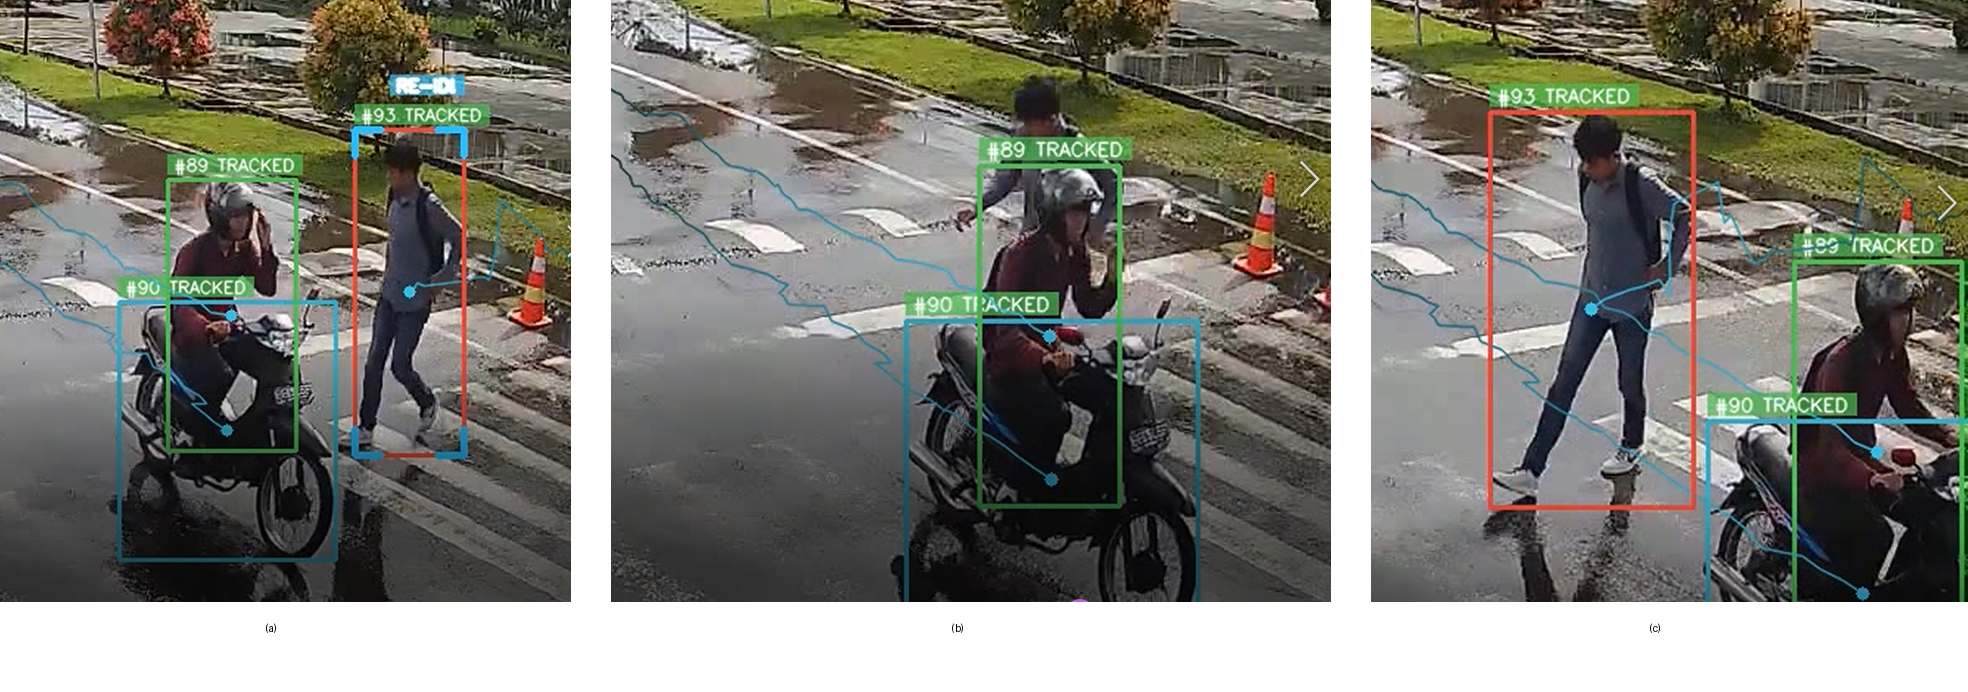
\includegraphics[width=0.95\textwidth]{gambar/figure_sequence_abc.png}
\caption{Sekuens visual ketahanan pelacakan ByteTrack saat menangani oklusi. Identitas \textit{Track ID} tetap dipertahankan secara persisten meskipun visibilitas objek sempat terhalang oleh kendaraan lain.}
\label{fig:occlusion-handling}
\end{figure}

% ============================================================
\subsection{Evaluasi Logika Spasial (IoA) dan Temporal (N-\textit{frame})}
\label{subsec:evaluasi-ioa-nframe}
% ============================================================

Mekanisme penyaringan bertingkat mereduksi deteksi mentah secara berlapis sebelum data dicatat sebagai pelanggaran. Pada pengolahan 3.001 \textit{frame}, deteksi awal sebanyak 9.544 disusutkan melalui seleksi objek, asosiasi identitas, filter spasial, filter temporal, dan deduplikasi. Tabel~\ref{tab:filtering-funnel} merinci hasil reduksi pada tiap tahap.

% --- ANALITIK ---
Pada Tabel~\ref{tab:filtering-funnel}, sistem hanya menyisakan 2 kejadian pelanggaran unik dari 9.544 deteksi mentah seluruh kelas (retensi 0,02\%), atau reduksi $801\times$ dari data kasar ke \textit{event} tervalidasi. Dari 1.602 deteksi \texttt{NO\_HELMET}, filter spasial IoA menggugurkan 1.567 deteksi (97,8\%) yang tidak memenuhi relasi spasial dengan sepeda motor. Selektivitas tinggi pada IoA mengindikasikan sebagian besar deteksi \texttt{NO\_HELMET} mentah berasal dari konteks non-berkendara, yaitu pejalan kaki, objek stasioner, atau \textit{false positive} model di area gerbang. Filter N-\textit{frame} kemudian menolak 10 dari 35 deteksi yang lolos IoA karena tidak memenuhi ambang konsistensi temporal (\textit{streak} $\geq$3 \textit{frame}), sehingga gangguan sesaat seperti bayangan atau pantulan cahaya tidak tercatat sebagai pelanggaran. Tahap akhir deduplikasi per-\textit{track} memadatkan 25 konfirmasi tingkat-\textit{frame} menjadi 2 \textit{event} unik, sehingga pelanggar yang sama tidak dihitung berulang dalam satu sesi. Kombinasi filter spasial, temporal, dan deduplikasi menaikkan kualitas data pelanggaran dan menekan \textit{false positive}, selaras dengan praktik pada sistem analitik transportasi berbasis video.

% --- EVIDENCE 1 ---
\begin{table}[htbp]
\centering
\caption{\textit{Filtering funnel}: Reduksi jumlah deteksi pada setiap tahap pipeline validasi pelanggaran (3.001 \textit{frame}).}
\label{tab:filtering-funnel}
\small
\setlength{\tabcolsep}{2pt}
\scriptsize
\begin{tabular}{p{1.2cm}p{2.0cm}p{2.0cm}p{2.0cm}p{2.0cm}}
\toprule
\textbf{Tahap} & \textbf{Deskripsi Proses} & \textbf{Jumlah Data} & \textbf{Tersaring} & \textbf{\% Retensi} \\
\midrule
0 & Deteksi mentah YOLO (semua objek) & 9.544 & --- & 100,0\% \\
1 & Seleksi objek target (\texttt{NO\_HELMET}) & 1.602 & 7.942 & 16,8\% \\
2 & Asosiasi identitas pelacakan (\textit{Track ID}) & 1.602 & 0 & 16,8\% \\
3 & Filter spasial IoA ($\geq$0,3 terhadap motor) & 35 & 1.567 & 0,37\% \\
4 & Konfirmasi temporal N-\textit{frame} (\textit{streak} $\geq$3 \textit{frame}) & 25 & 10 & 0,26\% \\
5 & Deduplikasi per-\textit{track} (\textit{Event} Unik) & \textbf{2} & 23 & \textbf{0,02\%} \\
\bottomrule
\end{tabular}
\end{table}
% ============================================================
\subsection{Karakterisasi Kecepatan (\textit{Throughput}) dan Latensi Infrastruktur Sistem}
\label{subsec:throughput-latency}
% ============================================================

Kinerja sistem pemrosesan video waktu nyata dinilai melalui dua metrik utama, yaitu \textit{throughput} (FPS) dan \textit{latency} (waktu tunda inferensi). Pengukuran dilakukan pada 3.001 \textit{frame} video secara berkelanjutan di perangkat CPU. Gambar~\ref{fig:fps-timeseries-evidence} menampilkan pola perubahan \textit{throughput} dan Tabel~\ref{tab:latency-decomposition} memuat rincian waktu proses tiap komponen.

% --- EVIDENCE 2 ---
\begin{figure}[htbp]
\centering
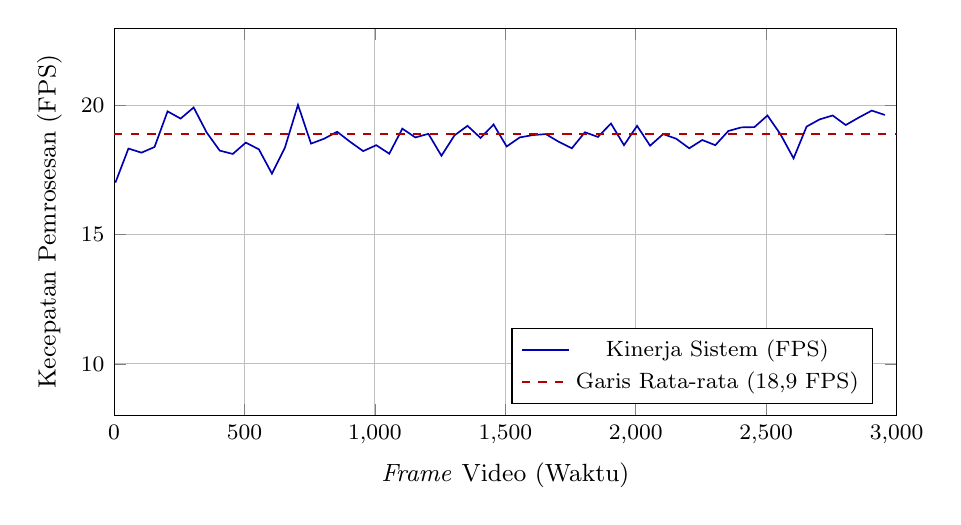
\begin{tikzpicture}
\begin{axis}[
  width=0.95\textwidth,
  height=6.5cm,
  xlabel={\textit{Frame} Video (Waktu)},
  ylabel={Kecepatan Pemrosesan (FPS)},
  xmin=0, xmax=3000,
  ymin=8, ymax=23,
  grid=major,
  grid style={line width=0.2pt, draw=gray!30},
  major grid style={line width=0.4pt, draw=gray!50},
  legend pos=south east,
  legend style={font=\footnotesize},
  tick label style={font=\footnotesize},
  label style={font=\small},
  title style={font=\small\bfseries},
]
% FPS time series (sampled every ~100 frames)
\addplot[blue!70!black, line width=0.6pt, mark=none] coordinates {
  (5,17.02) (55,18.34) (105,18.18) (155,18.40) (205,19.78)
  (255,19.50) (305,19.93) (355,18.96) (405,18.26) (455,18.13)
  (505,18.57) (555,18.31) (605,17.37) (655,18.38) (705,20.03)
  (755,18.53) (805,18.72) (855,18.99) (905,18.60) (955,18.24)
  (1005,18.47) (1055,18.14) (1105,19.11) (1155,18.77) (1205,18.91)
  (1255,18.06) (1305,18.85) (1355,19.22) (1405,18.75) (1455,19.27)
  (1505,18.42) (1555,18.77) (1605,18.86) (1655,18.90) (1705,18.60)
  (1755,18.35) (1805,18.97) (1855,18.79) (1905,19.31) (1955,18.47)
  (2005,19.22) (2055,18.45) (2105,18.90) (2155,18.72) (2205,18.35)
  (2255,18.67) (2305,18.47) (2355,19.02) (2405,19.16) (2455,19.17)
  (2505,19.62) (2555,18.89) (2605,17.96) (2655,19.19) (2705,19.47)
  (2755,19.62) (2805,19.25) (2855,19.54) (2905,19.81) (2955,19.64)
};
\addlegendentry{Kinerja Sistem (FPS)}
% Mean line
\addplot[red!70!black, dashed, line width=1pt, domain=0:3000] {18.9};
\addlegendentry{Garis Rata-rata (18,9 FPS)}
\end{axis}
\end{tikzpicture}
\caption{Dinamika \textit{throughput} pemrosesan \textit{pipeline end-to-end}. Kinerja terbukti konstan di kisaran 18,9 FPS tanpa mengalami indikasi \textit{memory leak} seiring berjalannya waktu.}
\label{fig:fps-timeseries-evidence}
\end{figure}

% --- ANALITIK ---
Pada Gambar~\ref{fig:fps-timeseries-evidence}, sistem mencatat rata-rata \textit{throughput} 18,9 FPS dengan pola stabil sepanjang pengujian. FPS di awal dan akhir pengujian tidak berbeda berarti, sehingga tidak ada indikasi degradasi akibat peningkatan penggunaan memori. Capaian sekitar 18 FPS pada perangkat tanpa GPU sudah berada di atas kebutuhan CCTV kampus yang umumnya beroperasi pada 10--15 FPS.

\begin{table}[htbp]
\centering
\caption{Rincian latensi pada setiap komponen perangkat lunak (dalam milidetik).}
\label{tab:latency-decomposition}
\small
\setlength{\tabcolsep}{4pt}
\begin{tabularx}{\textwidth}{>{\RaggedRight\arraybackslash}Xrrrr}
\toprule
\textbf{Komponen Pemrosesan} & \textbf{Rerata (ms)} & \textbf{P95 (ms)} & \textbf{Std. Dev} & \textbf{Porsi Komputasi} \\
\midrule
Inferensi Spasial YOLOv8 & 51,39 & 55,48 & 2,93 & \textbf{96,8\%} \\
Pelacakan ByteTrack & 1,62 & 2,80 & 0,82 & 3,1\% \\
Logika \textit{Filtering} Pelanggaran & 0,05 & 0,07 & 0,05 & 0,1\% \\
\midrule
\textbf{Total \textit{Latency} Sistem} & \textbf{53,06} & \textbf{57,52} & \textbf{3,23} & \textbf{100,0\%} \\
\bottomrule
\end{tabularx}
\end{table}
Pada Tabel~\ref{tab:latency-decomposition}, inferensi YOLOv8 mendominasi waktu proses (96,8\%) dan menjadi titik hambatan utama. Sebaliknya, ByteTrack dan modul validasi pelanggaran selesai di bawah 2 milidetik per \textit{frame}. Penambahan logika pelacakan dan validasi karena itu hanya membebani \textit{pipeline} dalam jumlah yang dapat diabaikan \cite{zhang2022bytetrack_eccv}. \textit{Latency} total berada pada kisaran 53 milidetik, sebuah orde puluhan milidetik yang masih responsif untuk pemantauan lalu lintas kampus berbasis aliran data hampir waktu nyata.

% ------------------------------------------------------------
\subsection{Reliabilitas dan Kapasitas Penyerapan Pesan (Apache Kafka)}
\label{subsec:evaluasi-kafka}
% ------------------------------------------------------------

Pengujian Kafka mengirimkan 500 paket peristiwa pelanggaran secara simultan ke topik \texttt{video.violations} yang dibagi ke dalam tiga partisi logis. Format pesan menggunakan \textit{JSON payload} dengan kompresi Snappy dan pengaturan \texttt{acks=all} untuk menjaga keutuhan pengiriman. Kunci partisi \textit{producer} dibentuk sebagai \texttt{camera\_id:track\_id} agar domain urutan pesan tetap konsisten per kamera. Ringkasan kinerja pengiriman pesan disajikan pada Tabel~\ref{tab:kafka-throughput}.

\begin{table}[htbp]
\centering
\caption{Metrik reliabilitas dan kecepatan transmisi (\textit{throughput}) pada klaster Apache Kafka.}
\label{tab:kafka-throughput}
\begin{tabular}{lr}
\toprule
\textbf{Parameter Evaluasi} & \textbf{Pencapaian Kinerja} \\
\midrule
Total Peristiwa Uji (\textit{Events Sent}) & 500 data JSON \\
Tingkat Keberhasilan Pengiriman & \textbf{100,0\%} (0 gagal) \\
Kecepatan Penyerapan (\textit{Producer Throughput}) & 11.485 pesan/detik \\
Volume \textit{Bandwidth} & 3,76 MB/detik \\
Ukuran Rata-rata \textit{Payload} & 335,6 Byte/pesan \\
Median waktu tunda transmisi (\textit{Latency}) & \textbf{2,65 milidetik} \\
\bottomrule
\end{tabular}
\end{table}
Pada Tabel~\ref{tab:kafka-throughput}, tingkat keberhasilan pengiriman mencapai 100\% tanpa pesan gagal, sehingga pengaturan \texttt{acks=all} mempertahankan keutuhan data saat terjadi gangguan jaringan sesaat. Pada sisi kecepatan, \textit{producer throughput} mencapai 11.485 pesan per detik dengan median latensi 2,65 milidetik. Nilai tersebut jauh di atas kebutuhan operasional harian sistem yang umumnya menghasilkan pelanggaran beberapa per menit. Margin kapasitas yang lebar tersebut memberi Kafka ruang menyerap lonjakan data tanpa kehilangan pesan. Pemisahan komponen melalui antrean Kafka mencegah pembentukan titik hambatan pada sistem video terdistribusi \cite{ayae2017video,kleppmann2017designing}, sehingga data tetap dapat diserap dan disimpan lebih dulu sebelum diproses lapisan analitik saat trafik masuk meningkat.

% ------------------------------------------------------------
\subsection{Dinamika \textit{Micro-Batch} dan Orkestrasi ETL (Apache Spark)}
\label{subsec:evaluasi-spark}
% ------------------------------------------------------------

Apache Spark Structured Streaming menjadi lapisan akhir \textit{pipeline}: mengonsumsi data dari Kafka, mendeduplikasi berbasis \texttt{event\_id} dengan \textit{watermark} 30 detik, memperkaya dimensi waktu, lalu memuat hasilnya ke PostgreSQL secara idempotent melalui mekanisme \textit{stage upsert}. Evaluasi pada bagian ini difokuskan pada dinamika \textit{micro-batch} dengan \textit{trigger interval} 10 detik sesuai konfigurasi implementasi. Tabel~\ref{tab:spark-microbatch} memuat bukti kuantitatif waktu pemrosesan pada beberapa batch aktif sebagai acuan analisis kinerja Spark pada beban berbeda \cite{zaharia2018structured}.


\begin{table}[htbp]
\centering
\caption{Dinamika latensi pemrosesan \textit{micro-batch} pada Apache Spark Structured Streaming (Interval: 10 detik).}
\label{tab:spark-microbatch}
\small
\setlength{\tabcolsep}{4pt}
\begin{tabularx}{\textwidth}{c>{\RaggedRight\arraybackslash}Xrrr}
\toprule
\textbf{ID Batch} & \textbf{Sifat \textit{batch}} & \textbf{Volume Data Masuk} & \textbf{Waktu Pemrosesan} & \textbf{Laju Eksekusi} \\
\midrule
Batch 0 & \textit{Empty / Idle} & 0 baris & 0 ms & 0 baris/detik \\
\textbf{Batch 1} & \textbf{Aktif (\textit{Spike})} & \textbf{50 baris} & \textbf{3.779 ms} & \textbf{13,2 baris/detik} \\
Batch 2--7 & \textit{Empty / Idle} & 0 baris & 0 ms & 0 baris/detik \\
\textbf{Batch 8} & \textbf{Aktif} & \textbf{20 baris} & \textbf{1.706 ms} & \textbf{11,7 baris/detik} \\
\textbf{Batch 10} & \textbf{Aktif} & \textbf{30 baris} & \textbf{1.705 ms} & \textbf{17,6 baris/detik} \\
\bottomrule
\end{tabularx}
\end{table}



Pada Tabel~\ref{tab:spark-microbatch}, pemrosesan \textit{micro-batch} Spark berjalan stabil pada \textit{trigger interval} 10 detik. Saat tidak ada data masuk (Batch 0 dan Batch 2--7), sistem berada pada kondisi \textit{idle} dengan waktu pemrosesan 0 ms. Saat beban melonjak, Batch 1 memproses 50 baris dalam 3.779 ms, sedangkan Batch 8 dan Batch 10 memproses 20 dan 30 baris dalam sekitar 1,7 detik. Seluruh durasi pemrosesan tetap di bawah batas 10 detik per siklus, sehingga tidak ada indikasi akumulasi antrean antar-batch.


Pengamatan ini sejalan dengan prinsip kerja Spark Structured Streaming: komputasi yang selesai di dalam jendela \textit{trigger} menjaga kontinuitas aliran data. Pemisahan proses \textit{ingest}, transformasi, dan pemuatan pada \textit{pipeline streaming} membuat sistem tetap tahan saat beban berubah antar-batch \cite{zaharia2018structured}. Pada skenario uji ini, sinkronisasi data dari CCTV hingga \textit{data mart} bertahan pada latensi operasional di bawah 10 detik, sehingga kebutuhan analitik lalu lintas kampus berbasis \textit{near real-time} terpenuhi.
% ============================================================
% ------------------------------------------------------------
\section{Implementasi \textit{Data Mart} Analitik Pelanggaran Helm}
\label{sec:data-mart}

Tahap hilir arsitektur ini mengonsolidasi aliran peristiwa (\textit{event stream}) menjadi wawasan operasional yang terukur dan dapat ditindaklanjuti. Subbab ini menguraikan tiga pilar transformasi data. Pertama, implementasi gudang penyimpanan analitik berbasis skema bintang (\textit{star schema}) pada PostgreSQL. Kedua, perancangan antarmuka dasbor interaktif (\textit{real-time dashboard}) menggunakan Grafana. Ketiga, evaluasi analitik atas rekaman operasional lapangan untuk memvalidasi peran sistem sebagai Sistem Pendukung Keputusan (\textit{Decision Support System}) dalam manajemen keselamatan kampus.
% ------------------------------------------------------------
\subsection{Implementasi \textit{Data Mart} Berbasis Skema Bintang (\textit{Star Schema})}
\label{subsec:implementasi-star-schema}
% ------------------------------------------------------------

Penyimpanan akhir data ekstraksi CCTV dibangun pada PostgreSQL menggunakan pendekatan skema bintang (\textit{star schema}). Aliran data pelanggaran dimuat ke tabel fakta pusat (\texttt{fact\_violations}) yang terhubung langsung dengan tiga tabel dimensi: \texttt{dim\_camera}, \texttt{dim\_violation\_type}, dan \texttt{dim\_time}. Gambar~\ref{fig:stardesign} menampilkan relasi kunci tamu (\textit{foreign key}) antar-tabel yang memisahkan metrik deteksi (probabilitas dan latensi pemrosesan) dari atribut deskriptifnya. Pemisahan ini mengikuti standar pemodelan dimensional yang menstrukturkan data sebelum tahap analisis.

% % --- EVIDENCE 1: Gambar ERD ---
% \begin{figure}[H]
% \centering
% \includegraphics[width=0.95\textwidth]{gambar/erd_data_mart.png}
% \caption{Realisasi fisik \textit{Entity Relationship Diagram} (ERD) dari \textit{Star Schema} pada PostgreSQL. Tabel \texttt{fact\_violations} memegang \textit{foreign key} yang merujuk pada dimensi waktu, kamera, dan jenis pelanggaran.}
% \label{fig:erd-physical}
% \end{figure}

Berbeda dengan evaluasi \textit{pipeline} pada Subbab~\ref{subsec:evaluasi-ioa-nframe} yang memakai potongan 3.001 \textit{frame}, bagian ini melaporkan eksekusi sistem pada rekaman operasional penuh. Pemuatan data (\textit{data loading}) ke \textit{data mart} dievaluasi memakai hasil ekstraksi \textit{pipeline} pemrosesan video CCTV Gerbang Utama Itera (\texttt{gate\_utama\_01}). Data terkumpul selama 10 jam operasional aktif pada hari kerja, pukul 07.00 hingga 17.00 WIB. Setelah ekstraksi dan transformasi, sistem memuat $113$ insiden pelanggaran berkendara tanpa helm secara persisten ke tabel fakta. Setiap baris terpetakan ke dimensi waktu (jam dan periode pagi, siang, sore) dan terhubung dengan dimensi kamera serta jenis pelanggaran.



Pada Tabel~\ref{tab:datamart-sample}, mekanisme penggabungan (\textit{join}) relasional berjalan sesuai rancangan arsitektur. Seluruh atribut kontekstual terekam tanpa anomali struktural, termasuk 12 rekaman yang memuat tautan bukti tangkapan layar (\textit{evidence image}). Pemuatan ini memperlihatkan \textit{pipeline} pendataan berhasil mentransformasi aliran data mentah (\textit{raw data}) berbasis video menjadi format basis data multidimensi. Validitas pemuatan tersebut menyiapkan \textit{star schema} sebagai fondasi agregasi dan kueri analitik lalu lintas pada tahap selanjutnya.
% --- EVIDENCE 2: Tabel Sampel Data ---
\begin{table}[htbp]
\centering
\caption{Contoh data hasil \textit{join} tabel fakta dan dimensi pada PostgreSQL berdasarkan rekaman operasional 10 jam.}
\label{tab:datamart-sample}
\footnotesize
\setlength{\tabcolsep}{3pt}
\renewcommand{\arraystretch}{1.15}
\begin{tabularx}{\textwidth}{>{\RaggedRight\arraybackslash}p{2.4cm} >{\RaggedRight\arraybackslash}X >{\RaggedRight\arraybackslash}p{3.0cm} >{\centering\arraybackslash}p{1.7cm} >{\centering\arraybackslash}p{1.4cm}}
\toprule
\textbf{Waktu Kejadian} & \textbf{Lokasi Sensor (Kamera)} & \textbf{Tipe Pelanggaran} & \textbf{Probabilitas} & \textbf{Latensi (ms)} \\
\midrule
2026-02-05 08:15:22 & Kamera Gerbang Utama 1 & Tanpa Helm & 85,2\% & 45,2 ms \\
2026-02-05 14:50:33 & Kamera Gerbang Utama 1 & Tanpa Helm & 65,4\% & 92,5 ms \\
2026-02-05 16:50:45 & Kamera Gerbang Utama 1 & Tanpa Helm & 82,3\% & 41,0 ms \\
\bottomrule
\end{tabularx}
\renewcommand{\arraystretch}{1.0}
\end{table}
\subsection{Visualisasi Dasbor Analitik Waktu Nyata (\textit{Real-Time Dashboard})}
\label{subsec:visualisasi-dashboard}

Lapisan presentasi (\textit{presentation layer}) diwujudkan sebagai dasbor interaktif berbasis Grafana. 


% --- EVIDENCE 1: Screenshot Grafana Overview ---
\begin{figure}[H]
\centering
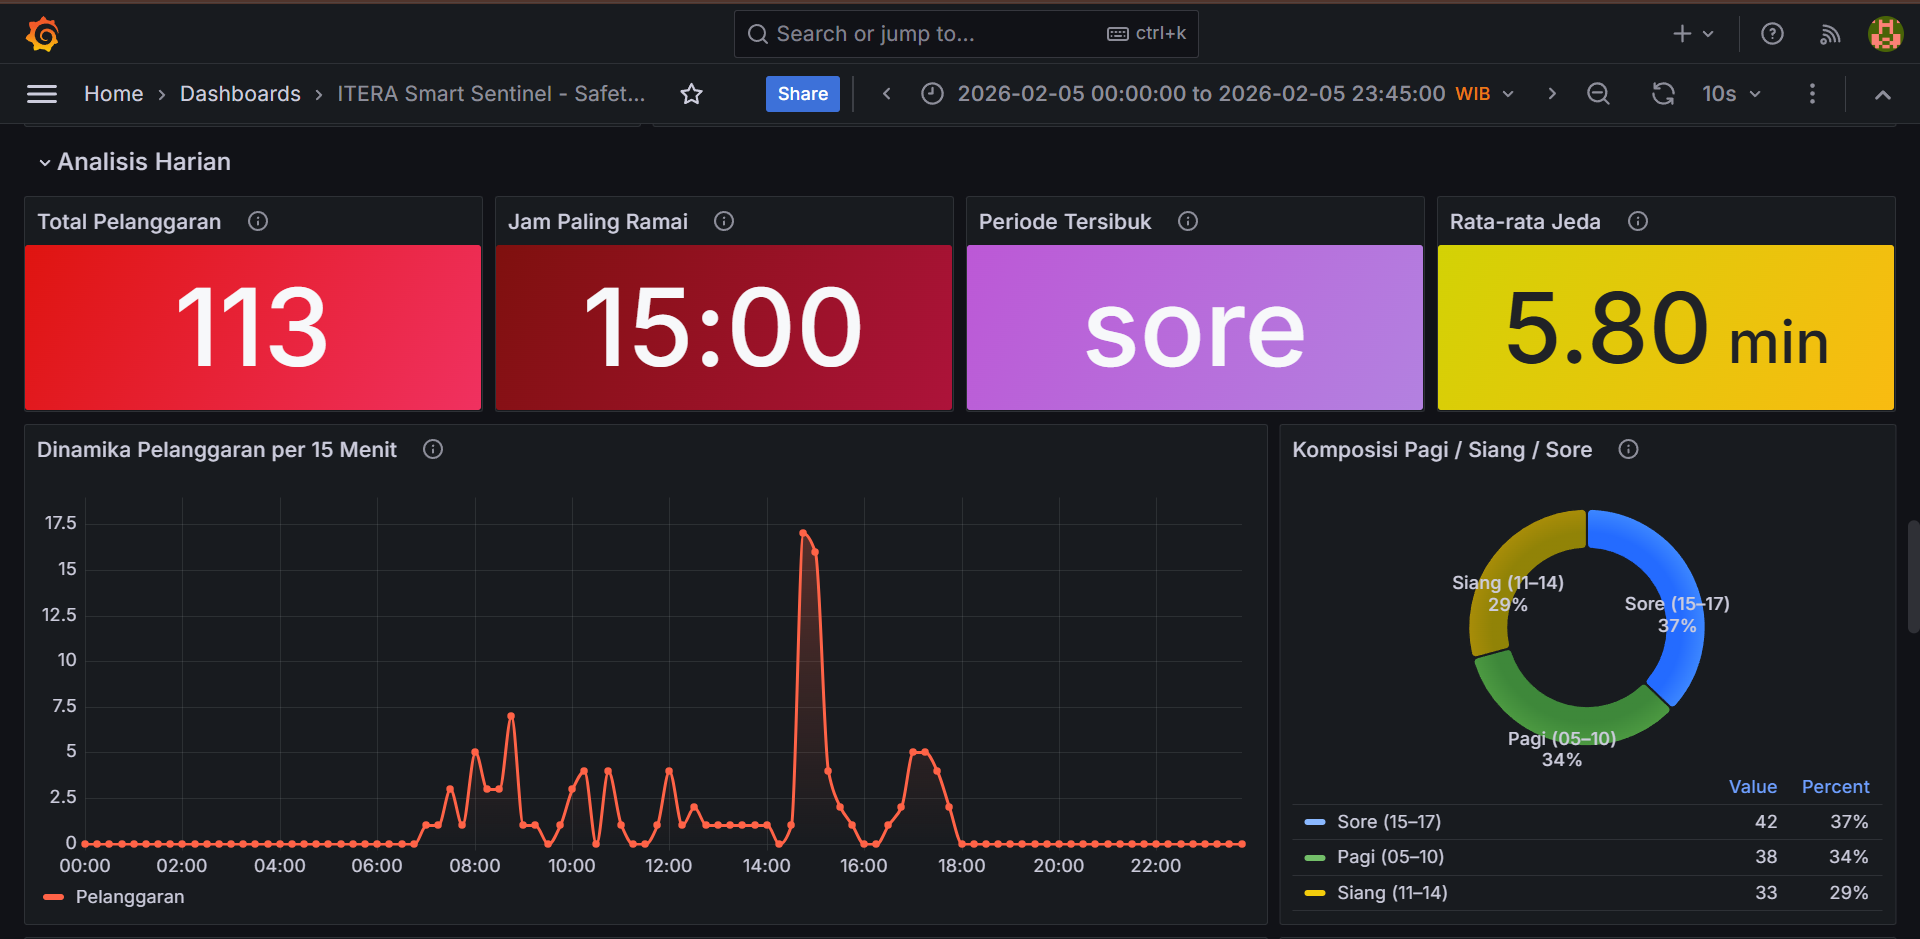
\includegraphics[width=0.95\textwidth]{gambar/grafana_kpi_overview.png}
\caption{Antarmuka utama Dasbor Grafana yang memvisualisasikan data operasional riil selama 10 jam. Sistem merender Indikator Kinerja Utama (KPI) serta dinamika pelanggaran per 15 menit berdasarkan ekstraksi CCTV.}
\label{fig:grafana-kpi-overview}
\end{figure}

Konfigurasi antarmuka membagi kebutuhan pengawasan ke dalam empat kategori panel analitik. Pembagian tersebut memisahkan fungsi pemantauan cepat, pelacakan tren waktu, evaluasi performa sistem AI, dan pemetaan distribusi spasio-temporal dalam satu alur kerja. Tabel~\ref{tab:dashboard-panels} merinci fungsi tiap kategori panel.


Pada pengujian antarmuka, pembaruan data dari skema bintang tersinkron dengan proses \textit{rendering} visual pada tiap panel. Sinkronisasi tersebut menempatkan arsitektur \textit{Business Intelligence} pada peran lapisan observasi yang siap dipakai untuk pemantauan kampus. Pembacaan pola temporal dan spasial secara analitis kemudian disajikan pada Subbab~\ref{subsec:analisis-data-lapangan}.

% --- EVIDENCE 2: Tabel Konfigurasi Panel ---
\begin{table}[htbp]
\centering
\caption{Daftar segmentasi panel pada dasbor analitik berdasarkan rancangan fungsional sistem.}
\label{tab:dashboard-panels}
\footnotesize
\setlength{\tabcolsep}{3pt}
\renewcommand{\arraystretch}{1.1}
\begin{tabularx}{\textwidth}{>{\RaggedRight\arraybackslash}p{4cm} >{\RaggedRight\arraybackslash}X}
\toprule
\textbf{Kategori Panel} & \textbf{Deskripsi Fungsi Visual dan Analitis} \\
\midrule
\textit{Indikator Kinerja Utama (KPI)} & Menyajikan ringkasan indikator secara cepat (\textit{single stat}) di area teratas, meliputi metrik Total Pelanggaran, Jam Paling Ramai, Periode Tersibuk, dan Rata-rata jeda waktu antar-pelanggaran. \\
\textit{Analisis Dinamika dan Tren Waktu} & Menganalisis fluktuasi \textit{time-series} melalui grafik garis per 15 menit, diagram batang akumulasi pelanggaran sepanjang hari (per jam vs kumulatif), dan komposisi waktu (Pagi/Siang/Sore). \\
\textit{Evaluasi Performa Sistem dan AI} & Merangkum kestabilan infrastruktur melalui grafik distribusi tingkat keyakinan AI (\textit{confidence level}) dan kecepatan deteksi (\textit{system latency}) saat dihadapkan pada variasi beban data. \\
\textit{Analisis Spasial dan Distribusi Temporal} & Memvisualisasikan lokasi anomali melalui matriks peta panas (\textit{heatmap}) temporal, sebaran \textit{hotspot} pada peta risiko geospasial, serta ringkasan agregat seperti Peringkat Top 5 Jam Tersibuk. \\
\bottomrule
\end{tabularx}
\renewcommand{\arraystretch}{1.0}
\end{table}

% ============================================================
\subsection{Analisis Wawasan Lapangan Berdasarkan Visualisasi Dasbor}
\label{subsec:analisis-data-lapangan}
% ============================================================

Implementasi \textit{Data Mart} mengekstraksi wawasan operasional dari data lapangan secara berulang. Data yang dipakai adalah hasil inferensi YOLOv8 dari aliran CCTV Kamera Gerbang Utama 1, bukan data sintetis. Pengamatan berlangsung selama 10 jam operasional pada hari kerja (07.00--17.00 WIB). Pembahasan berikut menguraikan keluaran tiap panel dasbor untuk menilai peran sistem sebagai pendukung pengambilan keputusan.

% ------------------------------------------------------------
\subsubsection{Dinamika Fluktuasi Interval Singkat (Deret Waktu 15 Menit)}
\label{subsubsec:analisis-dinamika-15m}

Pada resolusi temporal sempit, sistem mampu mengidentifikasi perubahan volume pelanggaran. Panel grafik garis ``Dinamika Pelanggaran per 15 Menit'' merangkum akumulasi log kejadian dari tabel fakta secara kontinu.

% --- EVIDENCE: Potongan gambar dinamika per 15 menit dari grafana_kpi_overview.jpg ---
\begin{figure}[htbp]
\centering
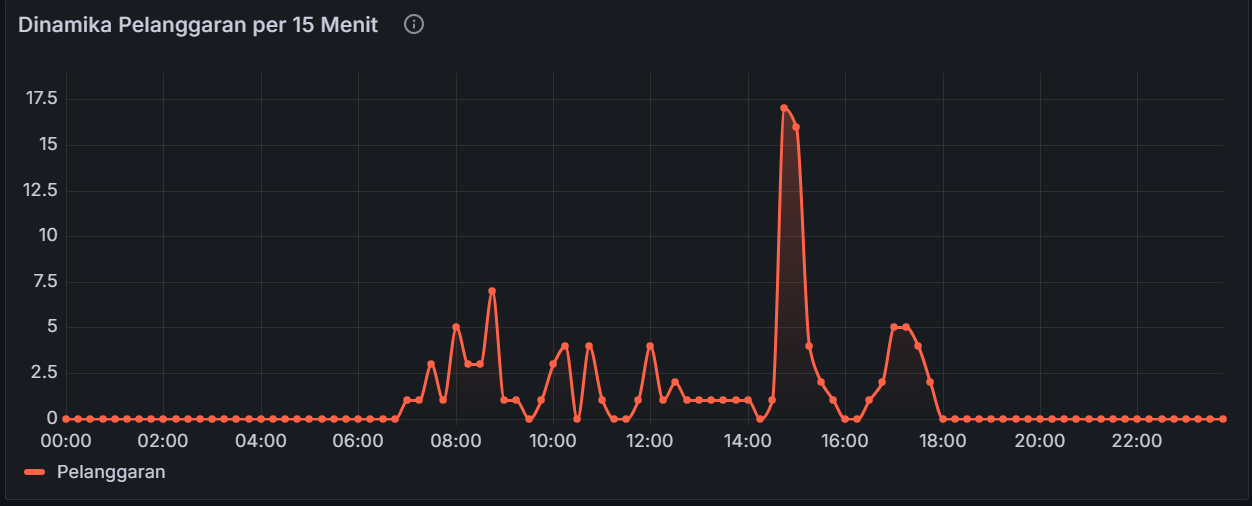
\includegraphics[width=0.90\textwidth]{gambar/grafana_dinamika_15m.png}
\caption{Visualisasi grafik deret waktu yang memetakan fluktuasi pelanggaran dengan resolusi 15 menit. Sistem merekam titik tertinggi (\textit{absolute peak}) sebesar 17 kejadian pada kuartal 14.45--15.00 WIB.}
\label{fig:grafana-dinamika-15m}
\end{figure}

Pada Gambar~\ref{fig:grafana-dinamika-15m}, kurva pelanggaran berfluktuasi mengikuti ritme aktivitas kampus. Nilai pelanggaran rendah pada rentang 09.00--10.00 WIB dan meningkat tajam pada jam pergantian kelas. Lonjakan tertinggi muncul pada kuartal 14.45--15.00 WIB dengan 17 kejadian per 15 menit. Observasi lapangan mengaitkan lonjakan sekitar pukul 15.00 WIB dengan dua kondisi yang berlangsung bersamaan: mobilitas pasca-hujan dan pertemuan arus mahasiswa yang keluar dan masuk kelas. Pola tersebut juga menyiratkan proses \textit{data ingestion} sinkron dan memadai sebagai landasan skema peringatan dini berbasis data waktu nyata.

% ------------------------------------------------------------
\subsubsection{Pola Akumulasi Harian dan Identifikasi Jam Tersibuk}
\label{subsubsec:analisis-akumulasi-jam}

Analisis agregat harian memetakan beban pelanggaran dari waktu ke waktu. Panel grafik Akumulasi Pelanggaran Sepanjang Hari dan matriks Top 5 Jam Tersibuk pada Gambar~\ref{fig:grafana-akumulasi} membandingkan tren kumulatif harian dengan persentase volume tiap jam operasional dalam susunan atas--bawah.

% --- EVIDENCE: Potongan gambar bar chart dan top 5 dari grafana_akumulasi_harian.png ---
\begin{figure}[htbp]
\centering
\includegraphics[width=0.95\textwidth]{gambar/grafana_akumulasi_harian.png}
\caption{Diagram batang ganda pada bagian atas menunjukkan pertumbuhan kumulatif vs insiden per jam, sedangkan matriks peringkat Top 5 jam tersibuk ditampilkan pada bagian bawah. Visualisasi menunjukkan dominansi kejadian yang terkonsentrasi pada dua periode utama.}
\label{fig:grafana-akumulasi}
\end{figure}

Pada diagram batang ganda (\textit{dual-bar chart}), tren pertumbuhan kumulatif (batang biru) bertambah secara asimetris. Dari total 113 kejadian, beban tertinggi tercatat pada pukul 15.00 WIB sebanyak 23 kejadian (20,4\% dari beban harian), diikuti pukul 14.00 WIB sebanyak 19 kejadian (16,8\%), dan kedatangan pagi pukul 08.00 WIB sebanyak 18 kejadian (15,9\%). Pemusatan tersebut membentuk distribusi bimodal yang kontras dengan jam perkuliahan reguler seperti 09.00 atau 11.00 WIB yang frekuensi pelanggarannya minim.

Frekuensi kumulatif yang tinggi pada rentang 14.00--15.00 WIB selaras dengan observasi lapangan. Titik kerawanan (\textit{vulnerability point}) jam tersebut bertepatan dengan peningkatan mobilitas mahasiswa setelah hujan lebat reda dan gelombang perpindahan saat transisi kelas sore.

Transformasi aliran video menjadi peringkat waktu memiliki implikasi operasional yang langsung. Dasbor memadatkan pemantauan harian menjadi indikator prioritas terukur. Pada level manajerial, unit pengamanan kampus dapat memakai persentase kontribusi waktu sebagai landasan objektif Sistem Pendukung Keputusan (\textit{Decision Support System}). Pemahaman pola anomali berbasis cuaca dan jadwal mengizinkan alokasi personel patroli dipusatkan pada jam berisiko tinggi sehingga pengawasan menjadi lebih preventif dan terarah.

% ------------------------------------------------------------
\subsubsection{Matriks Temporal dan Pemetaan Anomali Kepadatan}
\label{subsubsec:analisis-heatmap}

Pada resolusi waktu yang lebih granular, sistem basis data memproses kueri tabulasi silang (\textit{cross-tabulation}) untuk memetakan anomali kepadatan. Panel ``Peta Panas: Jam $\times$ Kuartal 15 Menit'' pada Gambar~\ref{fig:grafana-heatmap-real} memvisualisasikan distribusi frekuensi kejadian dengan gradasi intensitas warna dan total kumulatif per jam di sisi kanan matriks.

% --- EVIDENCE: Potongan gambar heatmap dari grafana_heatmap_real.png ---
\begin{figure}[htbp]
\centering
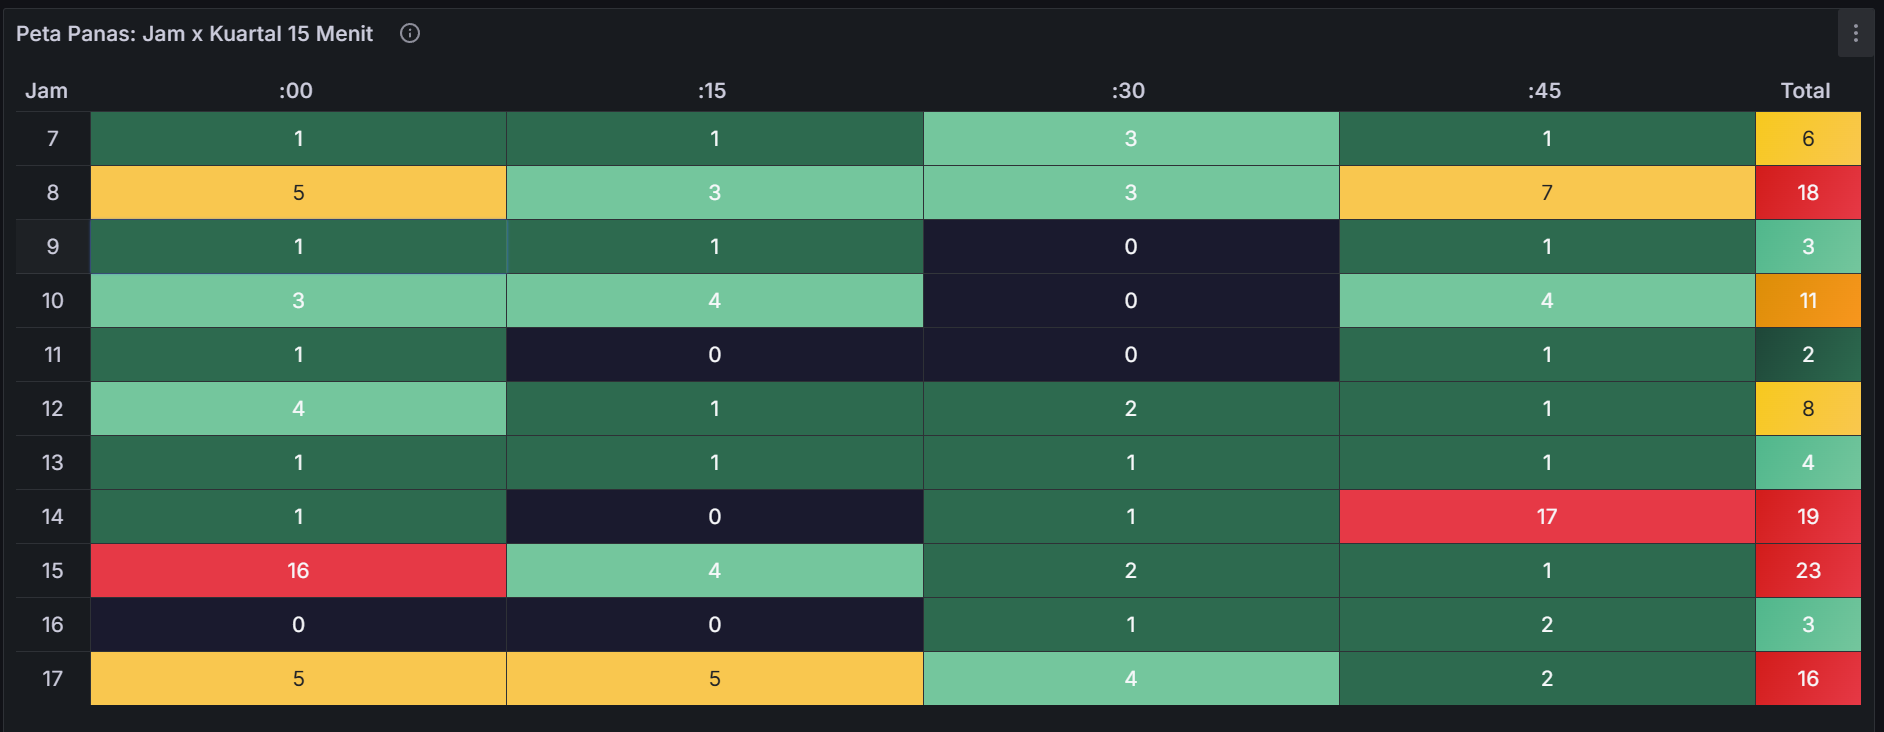
\includegraphics[width=1\textwidth]{gambar/grafana_heatmap_real.png}
\caption{Matriks peta panas yang membedah frekuensi kejadian ke dalam kuartal 15 menit. Warna merah pekat pada kolom :45 dan :00 menyoroti area kerawanan ekstrem yang terpusat pada sore hari.}
\label{fig:grafana-heatmap-real}
\end{figure}

Pada Gambar~\ref{fig:grafana-heatmap-real}, peta panas memperlihatkan fluktuasi waktu yang lebih rinci dibandingkan agregasi per jam. Konsentrasi merah pekat sebagai indikator kerawanan ekstrem (\textit{blind spot}) terpusat di jam 14 dan 15, khususnya kuartal :45 dan :00. Dasbor mencatat 17 kejadian pada kuartal 14.45--15.00 WIB dan 16 kejadian pada kuartal 15.00--15.15 WIB. Periode risiko tinggi karena itu berlangsung sekitar 30 menit di area gerbang kampus. Pola tersebut selaras dengan peningkatan arus kendaraan sesaat setelah hujan reda yang bertepatan dengan keluarnya mahasiswa dari kelas sore. Sebaliknya, pada jam perkuliahan aktif seperti pukul 11.00 dan 16.00 WIB, intensitas matriks mendekati nol kejadian.

% ------------------------------------------------------------
\subsubsection{Evaluasi Stabilitas Inferensi AI dan Infrastruktur Komputasi}
\label{subsubsec:analisis-stabilitas-ai}

Evaluasi fungsional tahap akhir menyorot ketahanan (\textit{robustness}) sistem saat lonjakan aliran data waktu nyata. Gambar~\ref{fig:grafana-evaluasi-sistem} menampilkan dua panel komparasi vertikal: volume objek pelanggaran (batang ungu) bersama indikator kesehatan model kecerdasan buatan (\textit{confidence}) dan kecepatan infrastruktur komputasi (\textit{latency}).


Pada grafik performa AI di bagian atas Gambar~\ref{fig:grafana-evaluasi-sistem}, tingkat keyakinan model bertahan konsisten meski volume pelanggaran melonjak. Saat lonjakan terjadi pada pukul 14.00 dan 15.00 WIB akibat mobilitas pasca-hujan dan pergantian kelas, rata-rata keyakinan (\textit{Avg Confidence}) tetap di kisaran 79,9\% sepanjang hari operasional. Batas bawah keyakinan (\textit{Min Confidence}) tertahan pada 51,2\% tanpa penurunan ekstrem (\textit{drop-off}). YOLOv8 karena itu tidak mengalami degradasi akurasi (\textit{model drift}) ketika kepadatan (\textit{crowd density}) dan oklusi antar-pengendara meningkat akibat cuaca. Pola serupa dilaporkan pada studi YOLOv8 untuk skenario lalu lintas kompleks yang juga mempertahankan performa tinggi pada deteksi pelanggaran helm waktu nyata \cite{deshpande2025helmetcv}.


% --- EVIDENCE: Potongan gambar confidence dan latency dari grafana_evaluasi_sistem.png ---
\begin{figure}[htbp]
\centering
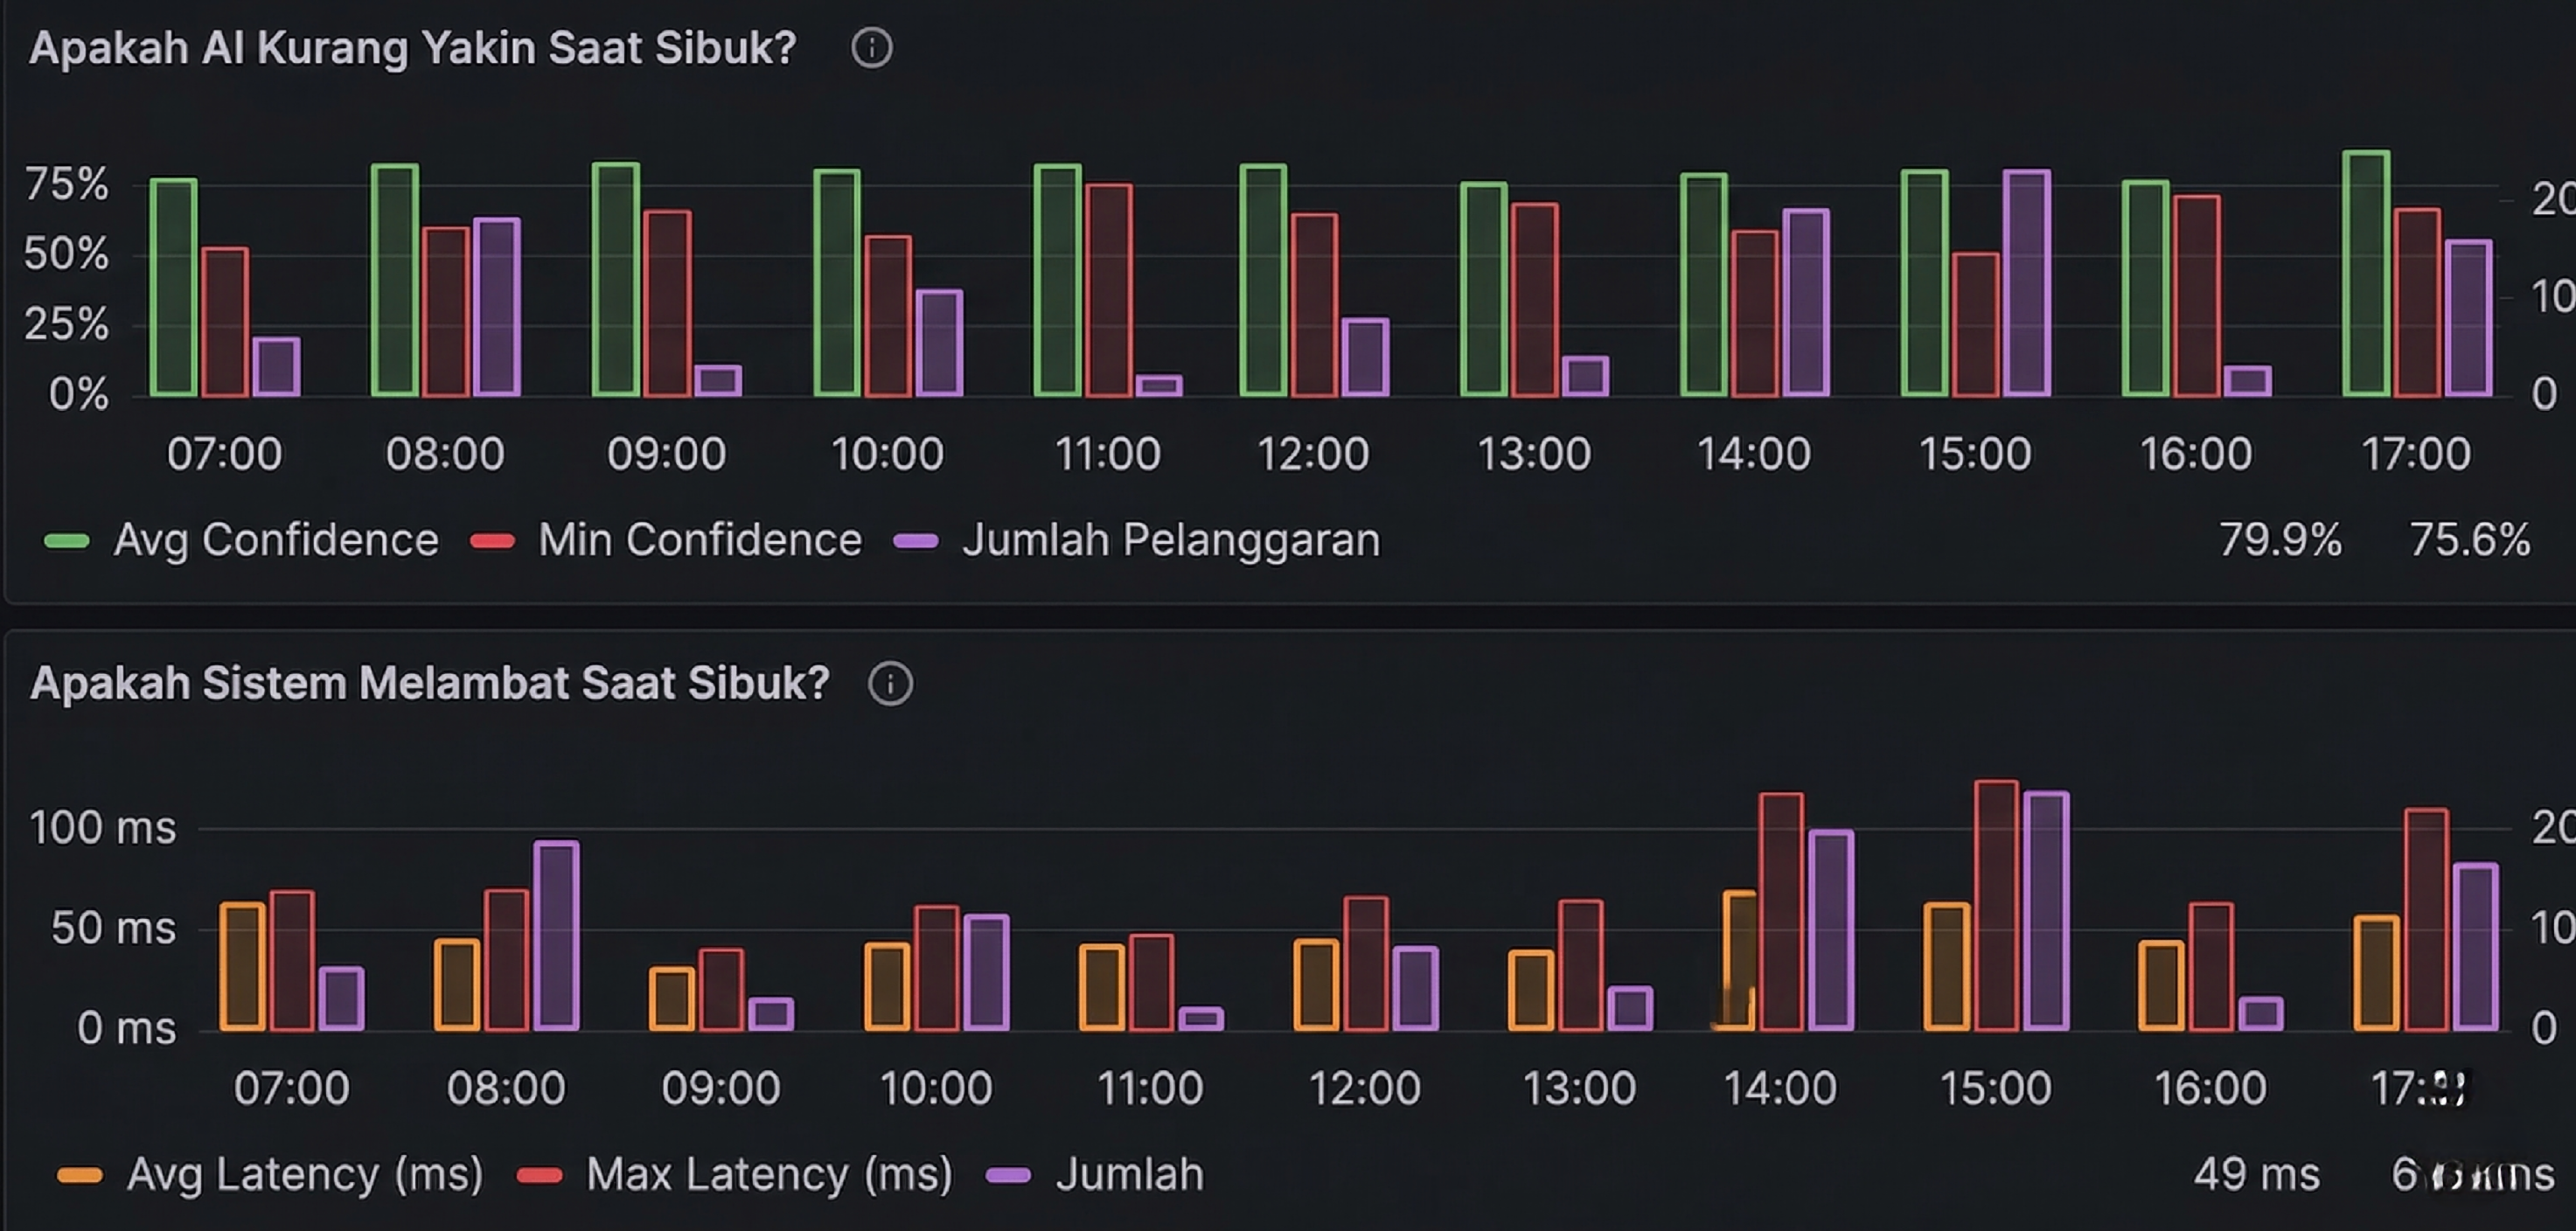
\includegraphics[width=1\textwidth]{gambar/grafana_evaluasi_sistem.png}
\caption{Komparasi performa arsitektur terhadap volume data dalam susunan atas--bawah. Grafik pada bagian atas menunjukkan stabilitas \textit{Confidence} AI, sedangkan grafik pada bagian bawah menunjukkan kestabilan \textit{Latency} server selama lonjakan beban lalu lintas terekam.}
\label{fig:grafana-evaluasi-sistem}
\end{figure}

Grafik bagian bawah memperlihatkan kinerja infrastruktur komputasi yang tetap stabil. Rata-rata latensi pemrosesan (\textit{Avg Latency}) tercatat 49 milidetik, termasuk saat beban meningkat pada bubaran kelas sore. Latensi maksimum (\textit{Max Latency}) sempat naik ke 124 milidetik pada beban puncak (23 kejadian pukul 15.00 WIB), tetapi masih di bawah batas operasional yang memicu \textit{system failure}. Tidak ada \textit{bottleneck} berarti selama lonjakan data. \textit{Big data pipeline} berbasis Apache Kafka dan Spark karena itu mampu menyerap \textit{spike} data secara asinkron, sehingga ekosistem \textit{Data Mart} memenuhi kebutuhan pemantauan kampus berkelanjutan.


% % Bab 5 penutup
% !TEX root = ../main.tex
\chapter{KESIMPULAN DAN SARAN}
\label{chap:kesimpulan}

% ============================================================
\section{Kesimpulan}
\label{sec:kesimpulan}
% ============================================================

Penelitian ini telah berhasil merancang, mengimplementasikan, dan mengevaluasi arsitektur sistem cerdas berbasis komputasi tepi (\textit{edge computing}) dan analitik data besar (\textit{big data analytics}) untuk pelacakan pelanggaran penggunaan helm di Institut Teknologi Sumatera (Itera). Berdasarkan evaluasi kinerja sistem secara menyeluruh, diperoleh tiga kesimpulan utama yang menjawab tujuan penelitian:

\begin{enumerate}[1.]
  \item  Model deteksi objek berbasis YOLOv8 berhasil dioptimalkan menggunakan dataset kustom CCTV kampus. Hasil evaluasi kuantitatif menunjukkan bahwa model beroperasi dengan keandalan tinggi, dibuktikan oleh capaian \textit{Mean Average Precision} (mAP@50) sebesar 91,4\% pada data validasi dan 90,0\% pada data uji. Keseimbangan marjinal antara \textit{precision} (87,5\%) dan \textit{recall} (86,5\%) mengonfirmasi bahwa model tidak hanya sensitif dalam melokalisasi target, tetapi juga presisi dalam membedakan kelas \texttt{MOTORCYCLE}, \texttt{DRIVER\_HELMET}, dan \texttt{DRIVER\_NO\_HELMET} di tengah berbagai distorsi visual dan kondisi pencahayaan luar ruang.

  \item Integrasi antara inferensi YOLOv8 dan algoritma pelacakan multiobjek ByteTrack terbukti berhasil mentransformasi deteksi piksel mentah menjadi aliran peristiwa (\textit{event stream}) yang terstruktur. Penerapan filter asosiasi spasial (\textit{Intersection over Area}) dan konfirmasi temporal (\textit{N-Frame}) secara efektif mengeliminasi deteksi positif palsu (\textit{false positives}) sebelum data ditransmisikan. Arsitektur pemrosesan tepi ini mencatat kinerja waktu nyata yang memadai tanpa dukungan GPU, dengan \textit{throughput} stabil pada 18,9 FPS dan latensi inferensi 53 milidetik. Selain itu, orkestrasi distribusi data melalui Apache Kafka (latensi transmisi 2,65 milidetik) dan Apache Spark Structured Streaming beroperasi secara asinkron tanpa memicu tekanan balik (\textit{memory backpressure}), memastikan ketahanan sistem saat menghadapi lonjakan aliran data.

  \item Perancangan \textit{data mart} berbasis skema bintang (\textit{star schema}) pada PostgreSQL terbukti efisien dalam menyajikan landasan komputasi untuk \textit{Online Analytical Processing} (OLAP). Pengujian operasional menggunakan data riil selama 10 jam (07.00--17.00 WIB) berhasil mengekstraksi wawasan operasional dari 113 kejadian pelanggaran aktual. Visualisasi pada dasbor Grafana secara presisi memetakan distribusi kepadatan bimodal, dengan anomali puncak absolut terekam pada pukul 14.45--15.15 WIB akibat korelasi faktor cuaca (pasca-hujan deras) dan transisi jadwal kelas. Implementasi infrastruktur ujung-ke-ujung (\textit{end-to-end}) ini berhasil memvalidasi fungsionalitas sistem bukan sekadar sebagai alat pendeteksi, melainkan sebagai instrumen Sistem Pendukung Keputusan (\textit{Decision Support System}) yang mentransformasi metode pengawasan UPT K3L Itera dari inspeksi reaktif menjadi penjagaan preventif yang terarah dan berbasis bukti (\textit{data-driven}).
\end{enumerate}

% ============================================================
\section{Saran}
\label{sec:saran}
% ============================================================

Meskipun sistem telah beroperasi secara fungsional sesuai dengan batasan penelitian, terdapat sejumlah peluang optimasi untuk pengembangan lebih lanjut agar arsitektur ini siap diterapkan pada skala produksi (\textit{production-grade}). Rekomendasi untuk penelitian mendatang adalah sebagai berikut:

\begin{enumerate}[1.]
  \item {Akselerasi Perangkat Keras pada Simpul Tepi (\textit{Edge AI}):}
    Beban komputasi inferensi spasial saat ini masih bertumpu pada Unit Pemroses Sentral (CPU). Untuk memperluas jangkauan sistem ke arsitektur multikamera (\textit{multi-camera surveillance}) dengan resolusi tingkat tinggi, disarankan untuk mendelegasikan beban inferensi pada akselerator perangkat keras spesifik (\textit{Hardware Accelerator}) seperti NVIDIA Jetson atau Google Coral Tensor Processing Unit (TPU). Pendekatan ini secara teoretis dapat mendongkrak \textit{throughput} melampaui 30 FPS dan mereduksi latensi operasional secara drastis.

  \item {Perluasan Ekstraksi Atribut Keselamatan dan Identifikasi Entitas:}
    Model visi komputer dapat dikembangkan lebih lanjut untuk mencakup deteksi bentuk pelanggaran sekunder yang berkontribusi pada risiko fatalitas, seperti kelebihan kapasitas penumpang motor (berbonceng tiga) atau penggunaan ponsel saat berkendara. Di samping itu, integrasi dengan subsistem \textit{Automatic License Plate Recognition} (ALPR) sangat direkomendasikan agar setiap aliran peristiwa dapat diikat langsung dengan identitas registrasi kendaraan pelanggar secara otonom.

\end{enumerate}

Secara keseluruhan, penelitian ini berkontribusi dalam menyajikan kerangka kerja arsitektur analitik video terintegrasi memadukan pembelajaran mendalam (YOLOv8), pelacakan multiobjek (ByteTrack), dan pemrosesan aliran data (Kafka--Spark) sebagai solusi pemantauan keselamatan lalu lintas cerdas yang efisien, skalabel, dan aplikatif di lingkungan perguruan tinggi.


% Daftar Pustaka
\phantomsection%<---
\addcontentsline{toc}{chapter}{DAFTAR PUSTAKA}
\sloppy
\printbibliography

% Halaman lampiran di tengah
\newpage
\phantomsection%<---
\addcontentsline{toc}{chapter}{LAMPIRAN}
\input{lainnya/lampiran-di-tengah.tex}

% Lampiran
\begin{appendix}

% !TEX root = ../main.tex
\chapter{LAMPIRAN}

\lampiran{Skema Data Warehouse}
\label{app:star_schema}

\subsubsection{Tabel Fakta (Fact Table)}


\begin{table}[H]
\centering
\caption{Tabel Fakta \textit{f\_violations}}
\label{tab:fact_violations}
\small\setlength{\tabcolsep}{4pt}\begin{tabularx}{\textwidth}{>{\raggedright\arraybackslash}p{0.27\textwidth}>{\raggedright\arraybackslash}p{0.20\textwidth}>{\raggedright\arraybackslash}X}
\toprule
\textbf{Kolom} & \textbf{Tipe Data} & \textbf{Deskripsi} \\
\midrule
\textit{violation\_id} & BIGINT (PK) & Kunci primer unik untuk setiap event pelanggaran. \\
\textit{timestamp\_fk} & BIGINT (FK) & Kunci asing ke \textit{dim\_time}. \\
\textit{camera\_fk} & INT (FK) & Kunci asing ke \textit{dim\_camera}. \\
\textit{violation\_type\_fk} & INT (FK) & Kunci asing ke \textit{dim\_violation\_type}. \\
\textit{track\_id} & VARCHAR(50) & ID unik objek yang dilacak (dari sistem deteksi). \\
\textit{duration\_in\_frame} & INT & Ukuran (measure) durasi objek dalam frame. \\
\bottomrule
\end{tabularx}
\end{table}

\subsubsection{Tabel Dimensi (Dimension Tables)}


\begin{table}[H]
\centering
\caption{Ringkasan Relasi Skema Bintang}
\label{tab:ringkasan-relasi-star-schema}
\small\setlength{\tabcolsep}{4pt}\begin{tabularx}{\textwidth}{>{\raggedright\arraybackslash}p{0.28\textwidth}>{\raggedright\arraybackslash}p{0.24\textwidth}>{\raggedright\arraybackslash}X}
\toprule
\textbf{Tabel} & \textbf{Kunci Utama} & \textbf{Relasi terhadap \textit{fact\_violations}} \\
\midrule
\texttt{dim\_time} & \texttt{timestamp\_pk} & Direlasikan melalui \texttt{timestamp\_fk} untuk menyediakan konteks waktu kejadian. \\
\texttt{dim\_camera} & \texttt{camera\_pk} & Direlasikan melalui \texttt{camera\_fk} untuk menyediakan konteks sumber kamera dan lokasi pemantauan. \\
\texttt{dim\_violation\_type} & \texttt{type\_pk} & Direlasikan melalui \texttt{violation\_type\_fk} untuk menyediakan konteks jenis pelanggaran yang terdeteksi. \\
\bottomrule
\end{tabularx}
\end{table}

\begin{table}[H]
\centering
\caption{Tabel Dimensi \textit{dim\_time}}
\label{tab:dim_time}
\small\setlength{\tabcolsep}{4pt}\begin{tabularx}{\textwidth}{>{\raggedright\arraybackslash}p{0.27\textwidth}>{\raggedright\arraybackslash}p{0.20\textwidth}>{\raggedright\arraybackslash}X}
\toprule
\textbf{Kolom} & \textbf{Tipe Data} & \textbf{Deskripsi} \\
\midrule
\textit{timestamp\_pk} & BIGINT (PK) & Kunci primer unik untuk dimensi waktu. \\
\textit{datetime\_full} & TIMESTAMP & Timestamp lengkap (YYYY-MM-DD HH:MI:SS). \\
\textit{hour\_of\_day} & SMALLINT & Jam dalam sehari (0--23). \\
\textit{day\_of\_week} & VARCHAR(10) & Nama hari (Senin, Selasa, ...). \\
\textit{date} & DATE & Tanggal. \\
\textit{month} & SMALLINT & Bulan dalam setahun (1--12). \\
\textit{year} & SMALLINT & Tahun. \\
\textit{is\_weekend} & BOOLEAN & Penanda (True/False) jika akhir pekan. \\
\textit{is\_exam\_period} & BOOLEAN & Penanda (True/False) jika masa ujian. \\
\bottomrule
\end{tabularx}
\end{table}

\begin{table}[H]
\centering
\caption{Tabel Dimensi \textit{dim\_camera}}
\label{tab:dim_camera}
\small\setlength{\tabcolsep}{4pt}\begin{tabularx}{\textwidth}{>{\raggedright\arraybackslash}p{0.27\textwidth}>{\raggedright\arraybackslash}p{0.20\textwidth}>{\raggedright\arraybackslash}X}
\toprule
\textbf{Kolom} & \textbf{Tipe Data} & \textbf{Deskripsi} \\
\midrule
\textit{camera\_pk} & INT (PK) & Kunci primer unik untuk kamera. \\
\textit{camera\_name} & VARCHAR(100) & Nama atau ID kamera (misal: \texttt{CCTV\_GERBANG\_A}). \\
\textit{location\_description} & VARCHAR(255) & Deskripsi lokasi pemasangan CCTV. \\
\textit{gps\_latitude} & DECIMAL(9,6) & Koordinat lintang. \\
\textit{gps\_longitude} & DECIMAL(9,6) & Koordinat bujur. \\
\bottomrule
\end{tabularx}
\end{table}

\begin{table}[H]
\centering
\caption{Tabel Dimensi \textit{dim\_violation\_type}}
\label{tab:dim_violation_type}
\small\setlength{\tabcolsep}{4pt}\begin{tabularx}{\textwidth}{>{\raggedright\arraybackslash}p{0.27\textwidth}>{\raggedright\arraybackslash}p{0.20\textwidth}>{\raggedright\arraybackslash}X}
\toprule
\textbf{Kolom} & \textbf{Tipe Data} & \textbf{Deskripsi} \\
\midrule
\textit{type\_pk} & INT (PK) & Kunci primer unik untuk jenis pelanggaran. \\
\textit{type\_name} & VARCHAR(50) & Nama pelanggaran (misal: \texttt{NO\_HELMET}). \\
\textit{description} & TEXT & Deskripsi detail dari aturan pelanggaran. \\
\bottomrule
\end{tabularx}
\end{table}

\lampiran{Kode Program dan Model melalui QR Code}
\label{app:qr_code_repo}

Lampiran ini menyediakan akses ke kode program dan model penelitian melalui \textit{Quick Response Code} (QR Code) pada Gambar~\ref{fig:qr-code-lampiran} dan tautan klikable \href{https://bit.ly/Lampiran-TA-EGGISATRIA}{lampiran digital}, sehingga pembaca dapat membuka berkas pendukung secara langsung.

\begin{figure}[H]
\centering

\includegraphics[width=0.45\textwidth]{gambar/qr_code_lampiran.png}
\caption{QR Code untuk mengakses lampiran digital yang memuat kode program dan model penelitian.}
\label{fig:qr-code-lampiran}
\end{figure}
\end{appendix}

\end{document}